% documentclass options:
\documentclass[11pt,
  a4paper,
  parskip=half, % This is some extra vertical space between paragraphs, the suggestion is 2cm which is really ugly, so we use what koma script gives us
  % you can also set it to full for even more space. But there is a bad tex style decision: parskip also changes the spacing between listitems such as
  % enumerate and itemize. For this purpose we include the enumitem package and set itemsep=.5em, of course you can change this
  BCOR=10mm, % BCOR is binding correction
  ngerman,
  % if you'd rather have a one sided thesis, add `oneside' to the documentclass
  % oneside,
  % ngerman is needed for hyphenation if the thesis contains parts written in German, switch order with english if you write mainly in English.
  % Remember to change order in the babel package (below) as well.
  % Last language is the preferred one.
  english]{scrbook}
\usepackage[ngerman, english]{babel} % If you write mainly in English change order to ngerman, english. Also change that in the documentclass options above.
% Include of titling must happen before \title etc.
% that's why it's not in setup.tex
\usepackage{titling}
\title{Ant Colony Optimization for Middle Voltage Grids}
\author{Paul Willi}
\usepackage[T1]{fontenc}
\usepackage{lmodern}
\usepackage{placeins}
\usepackage{amsmath}
\usepackage{tabularx}
\usepackage[gen]{eurosym}
\usepackage{svg}
% Change to your first examiner
% The ~ enables non sentence spacing after a period
\newcommand{\firstexaminer}{Prof.~Dr.~Christian Schindelhauer}
% Change to your second examiner, some undergraduate studies don't have a second examiner
% in this case just comment out the following line
\newcommand{\secondexaminer}{Prof.~Dr.~Christof \textbf{}Wittwer}
% Change to your adivers
\newcommand{\advisers}{Wolfgang Biener, Janis Kähler}

% include all packages and define commands in setup.tex

%------------------------------------------------------------------------------
%       package includes
%------------------------------------------------------------------------------
    % font encoding is set up for pdflatex, for other environments see
    % http://tex.stackexchange.com/questions/44694/fontenc-vs-inputenc
    \usepackage[T1]{fontenc}  % 8-bit fonts, improves handling of hyphenations
    \usepackage[utf8x]{inputenc}
    % provides `old' commands for table of contents. Eases the ability to switch
    % between book and scrbook
    \usepackage{scrhack}


    % ------------------- layout, default -------------------
    % adjust the style of float's captions, separated from text to improve readabilty
    \usepackage[labelfont=bf, labelsep=colon, format=hang, textfont=singlespacing]{caption}
    % With format = hang your caption will look like this:
    % Figure 1: Lorem ipsum dolor sit amet,
    %           consectetuer adipiscing elit.
    %           Ut purus elit, vestibulum
    % If you instead want
    % Figure 1: Lorem ipsum dolor sit amet,
    % consectetuer adipiscing elit. Ut purus
    % elit, vestibulum
    % change to format=plain
    \usepackage{chngcntr}  % continuous numbering of figures/tables over chapters
    \counterwithout{equation}{chapter}
    \counterwithout{figure}{chapter}
    \counterwithout{table}{chapter}

    % Uncomment the following line if you switch from scrbook to book
    % and comment the setkomafont line
    %\usepackage{titlesec}  % remove "Chapter" from the chapter title
    %\titleformat{\chapter}[hang]{\bfseries\huge}{\thechapter}{2pc}{\huge}
    \setkomafont{chapter}{\normalfont\bfseries\huge}

    \usepackage{setspace}  % Line spacing
    \onehalfspacing
    % \doublespacing  % uncomment for double spacing, e.g. for annotations in correction

    % ------------------- functional, default-------------------
    \usepackage{xcolor}  % more colors
    \usepackage{array}  % custom format per column in table - needed on the title page
    \usepackage{graphicx}  % include graphics
    \usepackage{subfig}  % divide figure, e.g. 1(a), 1(b)...
    \usepackage{amsmath}  % |
    \usepackage{amsthm}   % | math, bmatrix etc
    \usepackage{amsfonts} % |
    \usepackage{calc}  % calculate within LaTeX
    \usepackage[unicode=true,bookmarks=true,bookmarksnumbered=true,
                bookmarksopen=true,bookmarksopenlevel=1,breaklinks=false,
                pdfborder={0 0 0},backref=false,colorlinks=false]{hyperref}
    \usepackage{etoolbox} % if-else commands


    %==========================================
    % You might not need the following packages, I only included them as they
    % are needed for the example floats
    % ------------------- functional, custom -------------------
    \usepackage{algorithm,algpseudocode}
    \usepackage{bm}  % bold greek variables (boldmath)
    \usepackage{tikz}
    \usetikzlibrary{positioning}  % use: above left of, etc
    
    % Required for the ToDo list.
    \usepackage{ifthen}

    % Improves general appearance of the text
    \usepackage[protrusion=true,expansion=true, kerning]{microtype}
    \usepackage{enumitem}
    % Nicer font for pdf rendering.
    %\usepackage{lmodern}
    
    % For nicer looking tables.
    \usepackage{booktabs}

    % You don't need this, just for demonstration of a longer caption.
    \usepackage{lipsum}

%------------------------------------------------------------------------------
%       (re)new commands / settings
%------------------------------------------------------------------------------
    % ----------------- referencing ----------------
    \newcommand{\secref}[1]{Section~\ref{#1}}
    \newcommand{\chapref}[1]{Chapter~\ref{#1}}
    \renewcommand{\eqref}[1]{Equation~(\ref{#1})}
    \newcommand{\figref}[1]{Figure~\ref{#1}}
    \newcommand{\tabref}[1]{Table~\ref{#1}}

    % ------------------- colors -------------------
    \definecolor{darkgreen}{rgb}{0.0, 0.5, 0.0}
    % Colors of the Albert Ludwigs University as in
    % https://www.zuv.uni-freiburg.de/service/cd/cd-manual/farbwelt
    \definecolor{UniBlue}{RGB}{0, 74, 153}
    \definecolor{UniRed}{RGB}{193, 0, 42}
    \definecolor{UniGrey}{RGB}{154, 155, 156}


    % ------------------- layout -------------------
    % prevents floating objects from being placed ahead of their section
    \let\mySection\section\renewcommand{\section}{\suppressfloats[t]\mySection}
    \let\mySubSection\subsection\renewcommand{\subsection}{\suppressfloats[t]\mySubSection}



    % ------------------- math formatting commands -------------------
    % define vectors to be bold instead of using an arrow
    \renewcommand{\vec}[1]{\mathbf{#1}}
    \newcommand{\mat}[1]{\mathbf{#1}}
    % tag equation with name
    \newcommand{\eqname}[1]{\tag*{#1}}


    % ------------------- pdf settings -------------------
    % ADAPT THIS
    \hypersetup{pdftitle={\thetitle},
                pdfauthor={\theauthor},
                pdfsubject={Undergraduate thesis at the Albert Ludwig University of Freiburg},
                pdfkeywords={deep learning, awesome algorithm,  undergraduate thesis},
                pdfpagelayout=OneColumn, pdfnewwindow=true, pdfstartview=XYZ, plainpages=false}


    %==========================================
    % You might not need the following commands, I only included them as they
    % are needed for the example floats

    % ------------------- Tikz styles -------------------
    \tikzset{>=latex}  % arrow style


    % ------------------- algorithm ---------------------
    % Command to align comments in algorithm
    \newcommand{\alignedComment}[1]{\Comment{\parbox[t]{.35\linewidth}{#1}}}
    % define a foreach command in algorithms
    \algnewcommand\algorithmicforeach{\textbf{foreach}}
    \algdef{S}[FOR]{ForEach}[1]{\algorithmicforeach\ #1\ \algorithmicdo}

    % line spacing should be 1.5
    \renewcommand{\baselinestretch}{1.5}

    % set distance between items in a list, for more details see the
    % enumitem package: https://www.ctan.org/pkg/enumitem
    \setlist{itemsep=.5em}
    
    % use ra in your tables to increase the space between rows
    % 1.3 should be fine
    \newcommand{\ra}[1]{\renewcommand{\arraystretch}{#1}}

	% ToDo counters
	\usepackage{ifthen} %für whiledo-Schleife
	\newcounter{todos}
	\setcounter{todos}{0}
	\newcounter{extends}
	\setcounter{extends}{0}
	\newcounter{drafts}
	\setcounter{drafts}{0}

	% ------------------- marker commands -------------------
    % ToDo command
    \newcommand{\todo}[1]{\textbf{\textcolor{red}{(TODO: #1)}}\refstepcounter{todos}\label{todo \thetodos}}
	\newcommand{\extend}[1]{\textbf{\textcolor{darkgreen}{(EXTEND: #1)}}\refstepcounter{extends}\label{extend \theextends}}
	% Lighter color to note down quick drafts
	\newcommand{\draft}[1]{\textbf{\textcolor{NavyBlue}{(DRAFT: #1)}}\refstepcounter{drafts}\label{draft \thedrafts}}
	
	% microtype with lmodern, see https://tex.stackexchange.com/questions/75305/microtype-warning-with-lmodern-package-and-koma-script
	%\DeclareMicrotypeAlias{lmss}{cmr}

\begin{document}
    \pagestyle{empty} % no header and no page number
    % disable hyper links to remove warning "destination with same identifier"
    % this means within this section nothing can be referenced with a hyperlink
    \hypersetup{pageanchor=false}

    % enable/disable, depending on your chosen language
    
\begin{titlepage}
\begin{center}

\newcommand{\HorizontalLine}{\rule{\linewidth}{0.3mm}}

{\Large Master's Thesis}\\[1.3cm]


% _____________________________________________________________________________
\HorizontalLine \\[0.4cm]
% Write your title in a fancy way like this if you want to customize it, otherwise simply let tex do it for you
% \begin{spacing}{3}
%     {\huge \bfseries The Long, Long } \\
%     {\huge \bfseries Long Long} \\
%     {\huge \bfseries Title}\\
% \end{spacing}
{ \huge \bfseries \thetitle }
\HorizontalLine \\[1.5cm]
% _____________________________________________________________________________


{\Huge \theauthor} \\[2cm]


\begin{tabular}[hc]{>{\huge}l >{\huge}l}
  Examiner: & \firstexaminer \\[0.3cm]
  Advisers: & \advisers \\[1.2cm]
\end{tabular}
\vfill  % move the following text to the bottom

\Large {
    University of Freiburg\\
    Faculty of Engineering\\
    Department of Computer Science\\
    Chair/Laboratory for Thesis Templates\\[1cm]

    Mai 29\textsuperscript{th}, 2022\\
}
\end{center}
\end{titlepage}

\thispagestyle{empty}
% title page back
\ \vfill \ \\  % at least one space required before vfill
\
\textbf{Writing Period}            \smallskip{} \\
05.\,07.\,2016 -- 05.\,10.\,2016   \bigskip{} \\
\
\textbf{Examiner}                  \smallskip{} \\
\firstexaminer                     \bigskip{} \\
\
% If there is a second examiner include it
\ifdef{\secondexaminer}
	{
	% Include
	\textbf{Second Examiner}       \smallskip{} \\
	\secondexaminer                \bigskip{} \\
	\
	}
	{
	% No second examiner, ignore
	}
\textbf{Advisers}                  \smallskip{} \\
\advisers


    \pagestyle{plain} % remove chapter name from top, page number at the bottom
    % use \pagestyle{headings} for having the chapter on top of the pages
    % if you wang a more fancy header use \usepackage[automark,headsepline]{scrlayer-scrpage}
    % and read about it in the KOMA script documentation, https://www.ctan.org/pkg/koma-script
    \frontmatter  % roman page numbers
    % Copied from the official declaration from the examination office (typos fixed).
% Please double check the wording on their website and report changes.
% (https://www.tf.uni-freiburg.de/de/studium-lehre/a-bis-z-studium/dokumente/Declarationforthefinalthesis.pdf)

\chapter*{Declaration}

I hereby declare that I am the sole author and composer of my thesis and that no other sources or learning aids, other than those listed, have been used. Furthermore, I declare that I have acknowledged the work of others by providing detailed references of said work.  \newline
I hereby also declare that my Thesis has not been prepared for another examination
or assignment, either wholly or excerpts thereof.
\\[3\normalbaselineskip]
\begin{tabular}{p{\textwidth/2} l}
  \rule{\textwidth/3}{0.4pt}   &   \rule{\textwidth/3}{0.4pt} \\
  Place, Date                  &   Signature
\end{tabular}

    \chapter*{Abstract}
The transition to a carbon neutral energy supply is one of the greatest challenges of our time. The energy transmission system plays a major role in enabling renewable energy sources to efficiently participate in the electricity mix. The growing demand for electricity caused by the increase in electric vehicles and heat pumps among others requires expansion of the whole transmission system including the medium voltage level. The planning of grid expansion gets more difficult with increasing decentralized electricity generation and controllable loads. Therefore scientists developed automated planning tools to assist grid operators in planning their grid expansion. Ant colony optimization is one of the heuristic methods, which performed well for many use cases. This work focuses on target network planning of medium voltage grids using ant colony optimization. To complement previous research, this work considers information from low voltage level about potentially benefiting grid restructuring. Furthermore the presented method is tested and evaluated on a real world example using realistic as well as worst-case scenarios.
    \tableofcontents
    \listoffigures
    \listoftables
    \listofalgorithms
    \hypersetup{pageanchor=true}  % re-enable hyperlinking

    \mainmatter  % Arabic page numbers
    \chapter{Introduction}\label{chap:introduction}



Expansion of the electric grid is often necessary to cope with the growing demand for electricity. Additionally, the decentralized structure of power generation and the volatility of renewable energy sources pose challenges on the grid. New is also the possibility to control loads in form of batteries for electric vehicles for example.
...
Most use cases of network planning have their own specific properties and therefore the suggested automated solution must fit the respective problem. The distinction between high-, medium- and low-voltage levels of the grid are often used as a further classification for planning solutions. In addition to different nominal voltage levels they possess different topology constrains like the (n-1)-criterion for medium-voltage grids which must be considered by the algorithm. This categorization reduces the complexity of the problem but at the same time also reduces generality of application. ...

This work mainly focuses on target network planning for medium voltage grids. But additional information from low-voltage level about potentially useful transformer relocation is also considered.

Medium voltage grid expansion is especially relevant for rapid charging stations for electric cars. According to a report filed by the German federal network agency in 2021, the cost of the network expansion for the coming ten years amounts to 15.84 billion Euros where 9.47 billion (or 3.3 billion?! TODO: check paper again) are estimated for middle voltage grid (MV grid) expansion \cite{Ausbaubericht_2021_page14}. A smart MV grid expansion is therefore not only relevant for the future supply of electricity but also for public or private funding. \\

It is clear that the expansion of the electric grid is often necessary to cope with the growing demand for electricity. Additionally, the decentralized structure of power generation and the volatility of renewable energy sources pose challenges on the grid. New is also the possibility to control loads in form of batteries for electric vehicles for example. \\
Due to these new requirements and possibilities, also the planning of distribution grid expansion becomes more difficult. This makes is it harder for experts to rely on manual planning only. Instead, distribution system operators increasingly use automated optimization methods to find solutions of better quality. \\
According to \cite{rotering2013zielnetzplanung} network planning can roughly be categorized into “target network planning” and “expansion planning”, which correspond to the applied time horizon. Target network planning has a scope of a longer time horizon (ten years plus) and does not take existing grid infrastructure into account. It assumes that a new grid can be built from scratch and tries to find an optimal solution which fulfills all given requirements. This is typically used for the planning of new residential areas and long-term grid transformations. Network expansion on the other hand takes the existing grid infrastructure into account and tries to modify it in a way that it can cope with the more short- and mid-term demands (time horizon five to ten years). Mostly, target planning is done in a first step and afterwards the existing network is modified using expansion planning in the direction of the target network solution. In this work network planning generally refers to target network planning.\\

TODO: work in progress
    \chapter{Related Work}\label{chap:relatedwork}

From the introduction in the previous chapter it is clear that the expansion of the electric grid is often necessary to cope with the growing demand for electricity in context of the energy transition. In the literature exist different approaches for power distribution planning \cite{review}. They vary strongly in the methods they use, from exact numeric methods like non-linear- or dynamic-programming \cite{non_linear_programming, dynamic_programming} to heuristic methods like genetic algorithms \cite{genetic_algo}, tabu search \cite{tabu_search} and ant-colony-optimization. In addition to the different methods, they also differ in terms of side constraints which have to be fulfilled, as well as assumptions about the nature of the grid and inputs which need to be provided. Numeric methods are attractive because they produce exact and optimal solutions. Unfortunately, their performance is often times not good enough for most practical applications. Many challenges of grid planning involve NP-complete problems (e.g. related to the Traveling Salesman Problem) which leads to very long computational time of numeric methods even for strong machines. To reduce the run-time they need to simplify the problem to a great extend such that the results can not easily be translated to real world applications anymore. Due to this reason, heuristic methods seem to be more promising since they can find acceptable solutions even for NP-complete problems in polynomial time. This speed advantage makes them also applicable to more realistic scenarios without oversimplification. Unfortunately, heuristics can also introduce inaccuracies, which could lead to overconfidence in the produced solution. A thorough testing of the algorithm and an evaluation of the results is therefore necessary. This work uses a heuristic Ant Colony Optimization algorithm for network planning since they showed promising results in the past \cite{ant_system}\cite{bonabeau1999swarm}\cite{ant_coloy_system}.\\ Four sources were especially influential for the creation of this work and are presented in more detail in the upcoming sections. Afterwards, a brief overview of the new contributions to grid planning by this work is given.

\section{Dorigo et. al.}
Ant colony optimization methods are known to perform well on many grid planning problems. They were first introduced by Dorigo et. al. in 1996 in an algorithm called \textit{Ant System} \cite{ant_system}. \textit{Ant System} was tested and evaluated on the famous NP-complete Traveling Salesman Problem (TSP). Inspired by real ants astonishing ability of swarm intelligence to find short routes to sources of food Dorigo et. al. used artificial ants which can communicate and learn through pheromone trails left behind by ants of previous iterations.
The basic idea is that shorter paths to the food source will accumulate a higher density of pheromones, which leads to a convergence of most ants towards the shorter path. The artificial ants construct a technically valid solution and in a global pheromone update step the best solution is rewarded by an increase in pheromones whereas the other solutions are punished by a loss of pheromones.

One year later in 1997 Dorigo et. al. published an improved version called \textit{ant colony system} \cite{ant_coloy_system} which uses a local pheromone update in addition to the global pheromone update already used in the original algorithm. This local update removes pheromone on the paths already used by the ant, such that the next ant is more likely to chose a different path. This leads to a larger part of the search space being explored and reduces that chance of convergence towards a local optimum. The same procedure is also used in the algorithm of this work. A more detailed introduction to ant colony optimization algorithms with examples can be found in Chapter \ref{ACO}.\\

\section{Gebhard}
In 2021 Gebhard developed an algorithm in his thesis that uses ant colony optimization for expansion planning of low voltage grids called \textit{AntPower} \cite{gebhard2021expansion}. \textit{AntPower} combines conventional power line expansion with a reconfiguration of the power switches. Gebhard provides a great introduction into the planning of grids and the technical foundations for scholars outside electrical engineering like mathematics or computer science. Additionally, he gives a detailed description into how ACO is implemented in the context of grid planning. To evaluate the algorithm, real data of a village in rural Germany is used. His results show that the expansion plan generated by \textit{AntPower} is 60\% cheaper than an expansion plan obtained through conventional, manual planning based on expert knowledge and 64\% cheaper than the expansion plan generated using a local search algorithm.

\section{Rotering}
For the optimization of medium voltage grids via ACO, the dissertation of Rotering \cite{rotering2013zielnetzplanung} gives a great overview.
Rotering developed a procedure for medium voltage target planning using ant colony optimization which is also able to consider controllable loads and generators. In addition to network costs he also conducted an economic evaluation, which is part of the network design, but methodologically separate from the energy supply task of the network.\\
Rotering translates the electric grid into a graph and points out similarities between the medium voltage network problem and other optimization problems like the TSP. Since Ant Colony algorithms were specifically developed for the TSP Rotering opted to use them as an optimization tool. A crucial step in his procedure is the reduction of the potential connections between local network stations. He only considers edges of triangles created by the Delaunay triangulation as potential lines between networks stations. This dramatically reduces the search space and therefore reduces the runtime of the algorithm (further details in \ref{triangulation}). In addition, a triangle in itself already constitutes a ring structure which is important for the topological constraints of a MV grid (\textit{n-1 criterion}). Like Dorigo et. al. presented in \cite{ant_coloy_system}, Rotering uses a local and a global pheromone update for his algorithm. After the construction of a legal network design Rotering uses additional optimization methods to further improve the solution. He evaluates the his procedure on two MV grids and receives promising results.



\section{Zeller}
Zellers thesis about the planning of medium voltage grids via ACO serves as the basis for this work. The presented ACO algorithm \textit{APMV} is s a further development of the algorithm Zeller presents in \cite{zeller2021planung}. Zeller already uses some concepts like the Delaunay triangulation, a local and global pheromone update and pheromone evaporation in his algorithm. Zeller also considered special cases originating from the triangulation which could lead to faulty networks (called \textit{back-and-forth} cases). They are explained in further detail in \ref{backandforth}. In these cases Zeller extended and optimized the procedure to build valid solutions. Besides a practical analysis and a parameter study he conducted a theoretical analysis and provided several proofs to further legitimize the procedure. He showed, that given enough runtime the algorithm would always find the global optimum and that all buses would be connected. Additionally Zeller showed that the topological constraints would always be fulfilled. For evaluation of the developed algorithm Zeller used manually built synthetic grids with sizes of 5 to 30 nodes.

\newpage
\section{New contributions}
This work contributes to grid planning via ACO in the following ways:
\begin{enumerate}
	\setlength\itemsep{-0.5em}
	\item An improved algorithm for optimizing medium voltage grids called \textit{Ant-Power-Medium-Voltage} is presented.
	\item The algorithm is tested and evaluated on a real world cross-voltage grid.
	\item Cases, which previously lead to faulty network structures are intercepted.
	\item A parameter study to find the algorithms best performance is conducted.
\end{enumerate}

Regarding grid planning, so far in the literature many methods for grid planning are provided without testing and evaluating them on real world examples. Scientific research however, is only useful if it can be converted into an improvement of the practical application. Therefore, the aim of this work is to use the algorithm to optimize a real world cross-voltage grid and evaluate its performance. This grid is taken from a village which is located in rural Germany and and resembles a typical application example.\\
Besides applying existing research on a real world example, this work also presents an ACO algorithm with several improvements. Firstly, the accuracy of the cost function is increased by several measures. Secondly, the laying of new lines is done alongside streets to make more realistic estimations. Thirdly, overlapping rings in the network are handled in a sensible way. And lastly, cases which previously lead to faulty network structures are intercepted.



%to combine different methods to gain better overall results. Thus, the algorithm uses information from the low voltage level about potentially benefiting transformer modifications. It could be useful from the perspective of the low voltage level to relocate, add or delete a transformer to reduce costs or load flow violations. This method has been developed and evaluated by Verheggen \cite{verheggen2016kombinierte} and implemented by John in \cite{robert_john}. However, restructuring the transformers has an influence on the middle voltage level and therefore gains for the low voltage level have to be weighed out with potential losses for middle voltage level. \\







    \chapter{Background}\label{chap:background}
The upcoming chapter gives a basic description of electric grids and their structure. Afterwards, the functionality of ACO and its application to grid planning is presented. The goal is to provide sufficient background information for the understanding of the presented algorithm and its evaluation (i.e. for scholars of computer science or mathematics without previous knowledge about electric grids).

\section{Electric Grids}
An electric grid is the infrastructure, which enables the distribution of electric energy. Important components of a grid are the following.

\subsection{Components}\label{sec:components}

\textbf{Sources}: At sources electricity is fed into the electric grid (power plants, wind turbines, solar-panels etc.).

\textbf{Loads}: At loads electricity is subtracted from the grid (households, factories etc.).

\textbf{Lines}: Transmission lines connect sources and loads and transport the electricity.

\textbf{Buses}: A bus is a connection point between two lines or more. Loads and sources can be coupled to a bus but it can also be a mere connection point.

\textbf{Transformers}: Transform the voltage from one voltage level to another. A transformer can therefore also be seen as a generator or source within a certain voltage level. It functions as a connection between the different voltage levels of the grid.

\textbf{Switches}: Enable the opening and closing of connections between different branches of the grid. They are used cut off electricity from a branch in case of an emergency or to supply electricity to the consumer via an alternative route (n-1 criterion).

\textbf{Storage Units}: Enable the storage of energy (via pumped storage hydroelectricity, batteries, hydrogen etc.). 


\textbf{Transformers}: Transform the voltage from one voltage level to another one. A transformer therefore can also be seen as a generator or source from within a certain voltage level.

(\textbf{Slack bus}: In power flow studies, the slack bus is used to provide for system losses by emitting or absorbing active and reactive power to and from the system. It is usually located at the transformer connecting to the higher voltage level.)

\subsection{Structure}
To increase efficiency, the grid is usually separated into three different voltage levels: high-(HV), medium-(MV) and low-voltage (LV).

\textbf{HV grids} connect big power plants and transformer stations of underlying medium-voltage (MV) grids. They usually operate at voltages reaching from 110 to 380 kV. Their structure is more meshed to build up redundancy for safety.

\textbf{MV grids} connect smaller power plants, factories and transformer stations to the low-voltage (LV) level. They operate at around 10 to 20 kV and are required to fulfill the \textit{n-1 criterion}. So if one component of the MV grid fails, there is at least one built in redundancy to keep the grid functional.

\textbf{LV grids} mostly transfer electricity from the transformer stations to the households. Due to the increasing decentralized feedin of electricity the LV grid also needs to be capable of transferring energy between households. They usually operate at voltages of 0.4 kV.\\


\begin{figure}[h]
	\begin{centering}
		{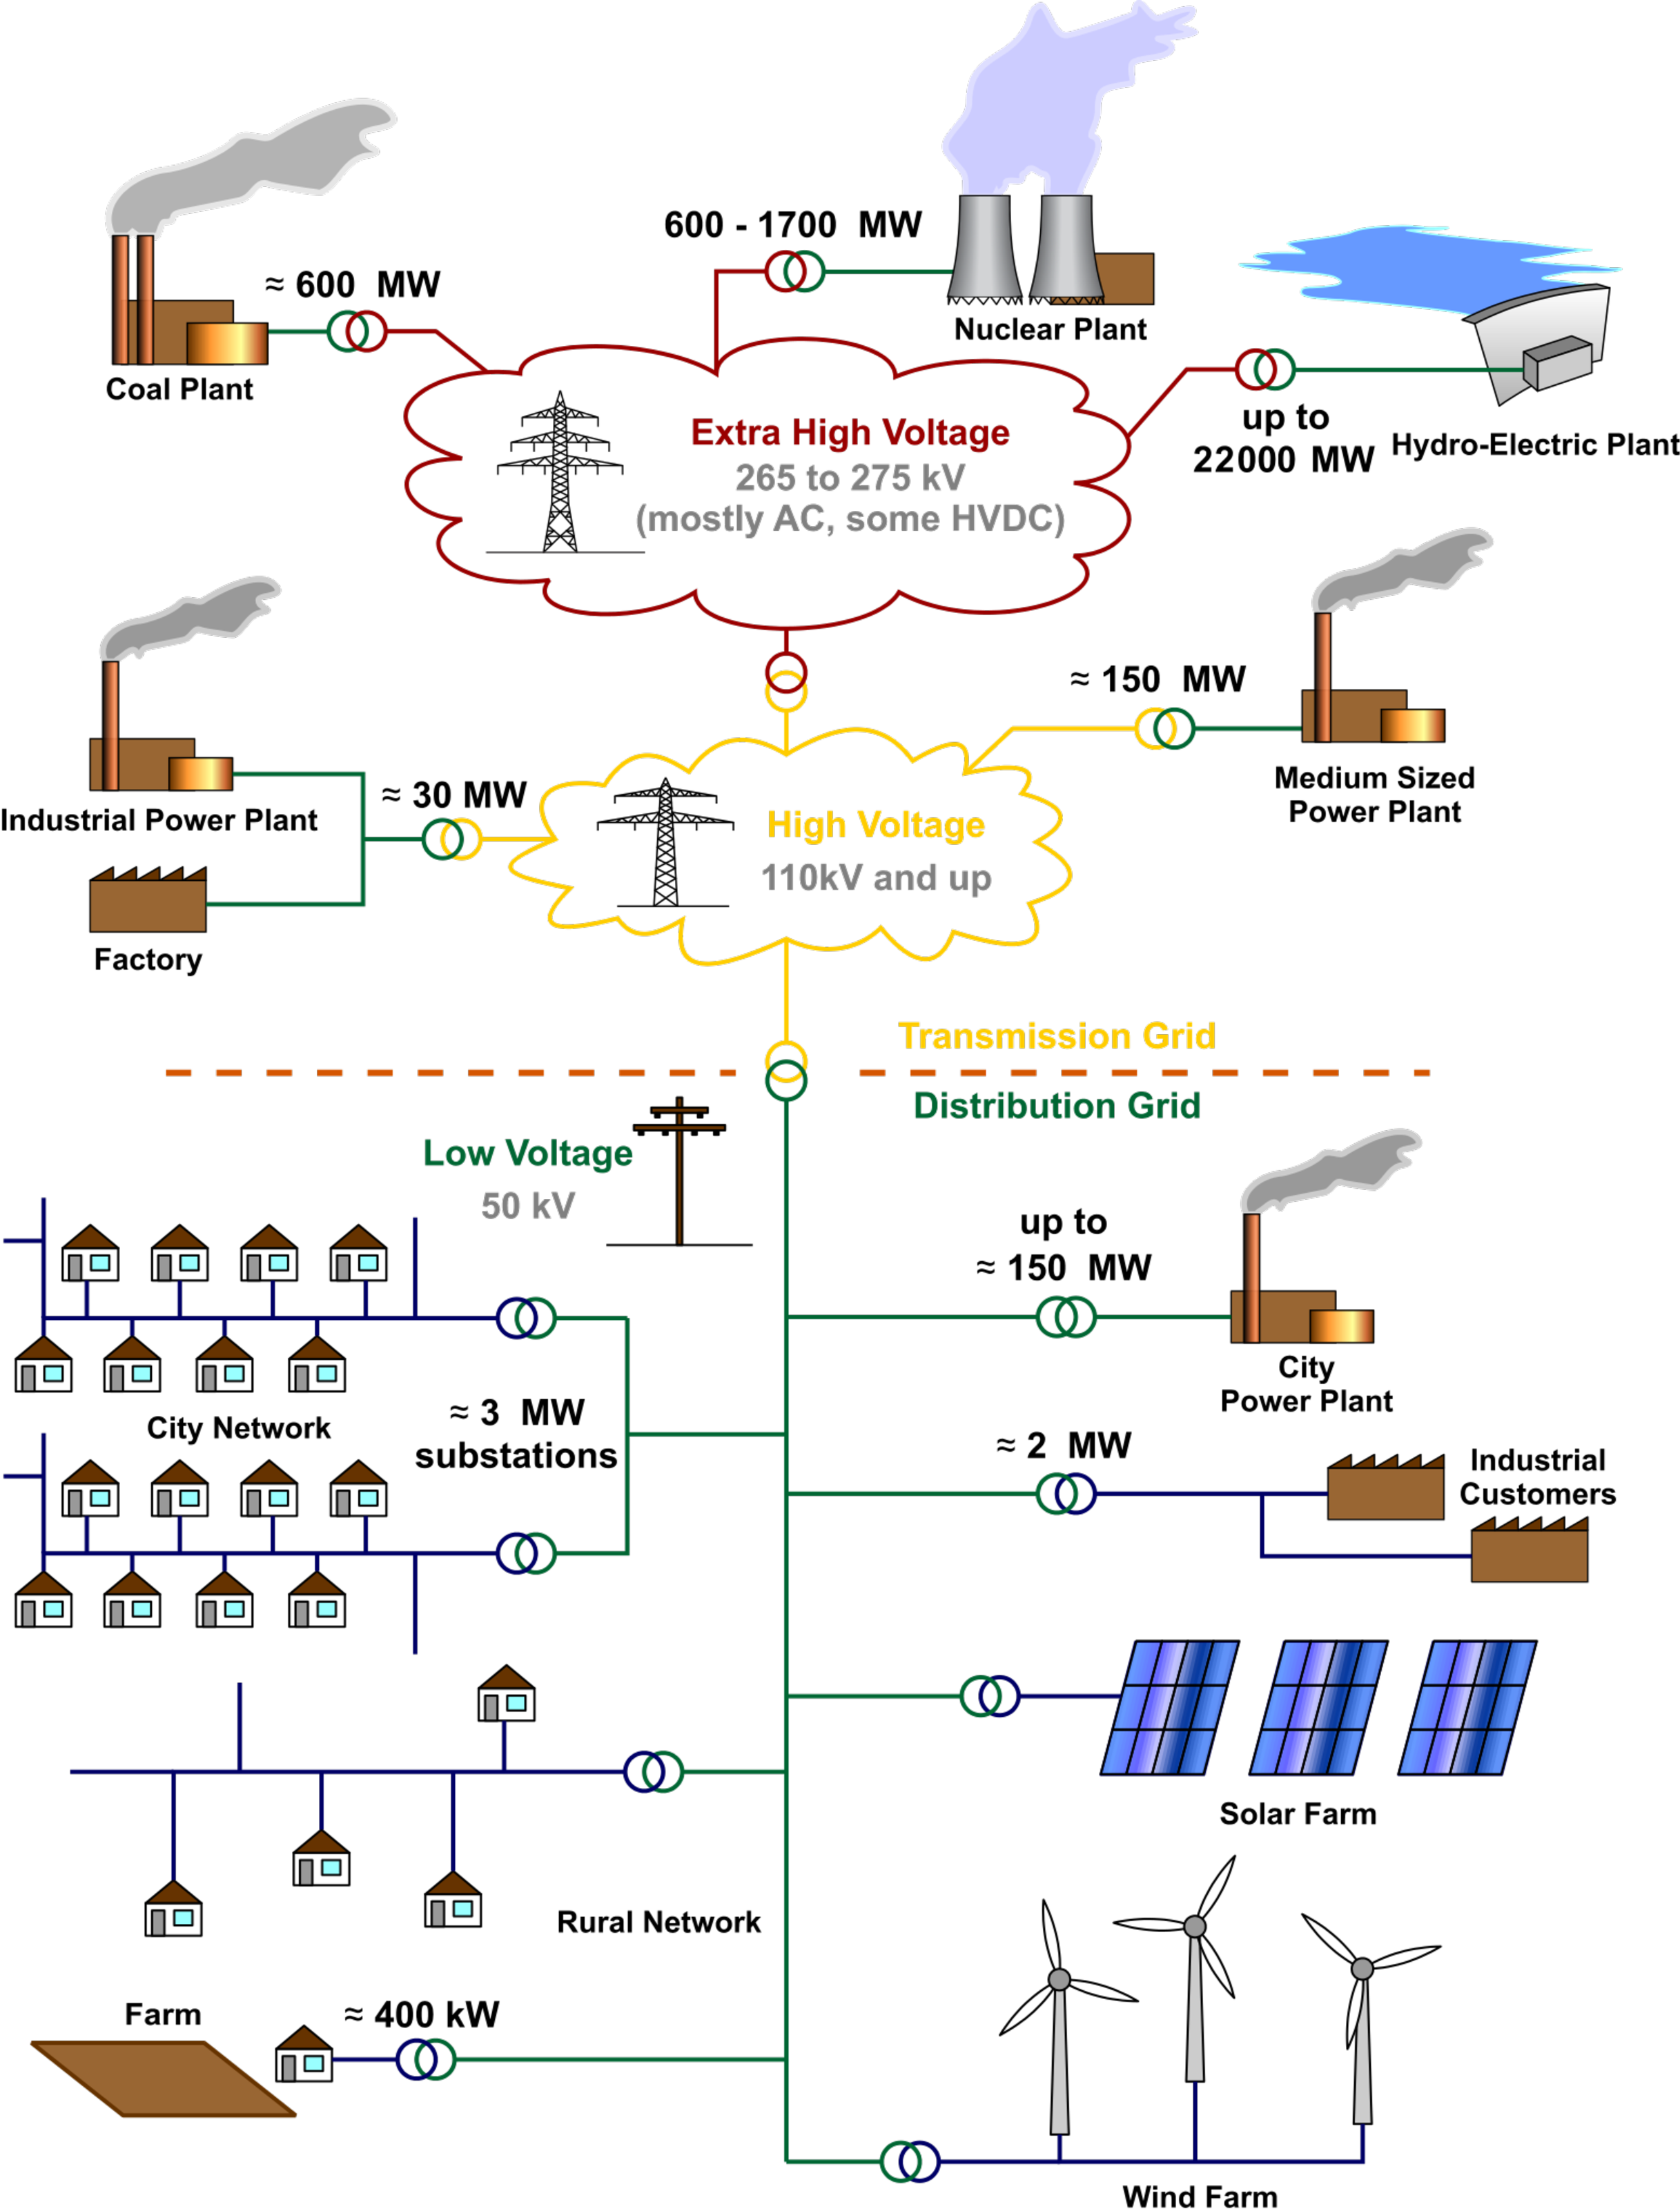
\includegraphics[scale=0.27]{figures/background/grid_schematicc.pdf}}
		\caption[Schematic depiction of the electricity grid]{Schematic depiction of the electricity grid common in Germany. Source: https://commons.wikimedia.org/wiki/File:Electricity$\protect\_$Grid$\protect\_$Schematic$\protect\_$English.svg}
		\label{fig:schematic_grid}
	\end{centering}
\end{figure}



\section{Ant Colony Optimization}\label{ACO}
ACO is inspired by the astonishing ability of real ants to find short paths between their nest to sources of food. Ants are mostly blind and coordinate their movements using pheromones, which they leave behind on the trails they use. Ants are able to sense the pheromones and tend to follow paths with a higher concentration of the messenger substance. Ants, which probabilistically follow the paths with higher pheromone concentration, again leave behind pheromones, which increase the chance of other ants to also follow this trail. Over time, this leads to a convergence of ants to follow the path with the highest pheromone concentration.

\subsection{The Double Bridge Experiment}

The following example is based on experiments Deneubourg et al. conducted with Argentine ants in 1990 \cite{deneubourg1990self}. The ants are placed at the starting location and two paths of different length connect them to a source of food.
\begin{figure}[h]
	\begin{centering}
		{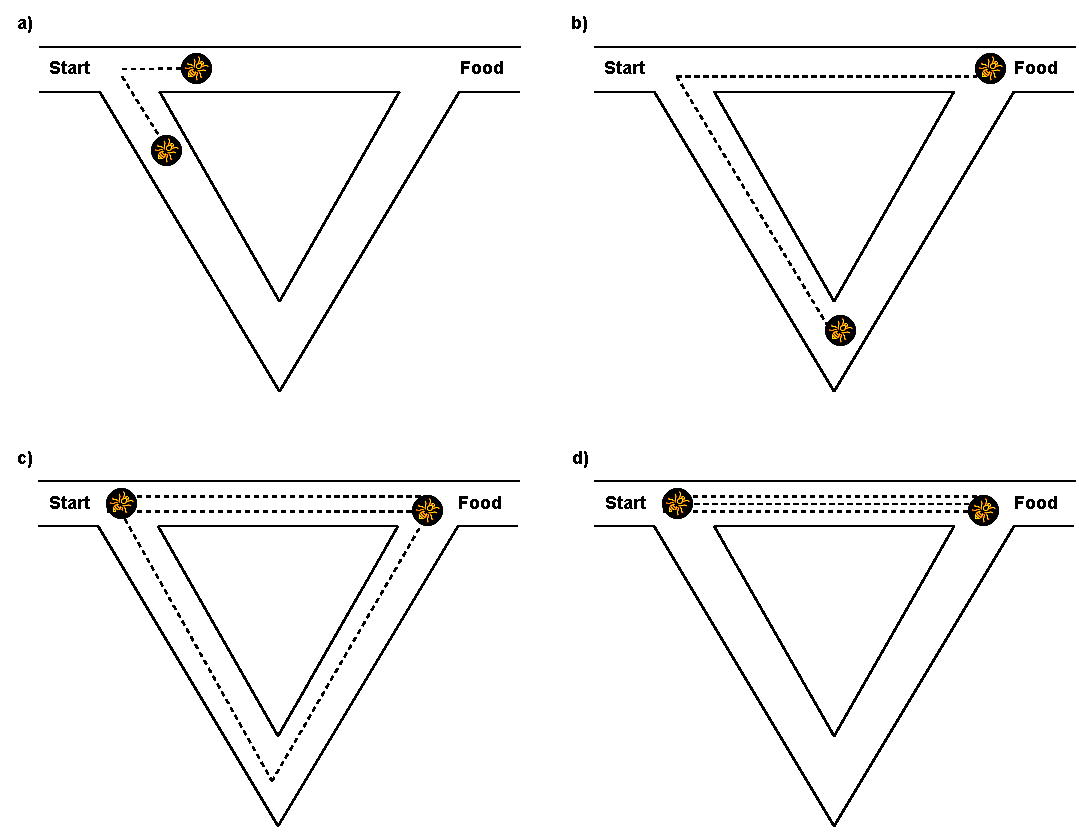
\includegraphics[scale=0.8]{figures/background/aco_double_bridge.pdf}}
		\caption{Double Bridge Experiment. Two paths of different length lead from the start to the food source.}
		\label{fig:double_bridge}
	\end{centering}
\end{figure}

As shown in \ref{fig:double_bridge}, at the beginning of the experiment the ants decide randomly which path they choose, since no pheromone has been distributed yet (a). Because one path is shorter, the ants who chose this path arrive at the food source earlier (b). On the way back, there only exists pheromone on the shorter path, which leads to a higher chance of ants choosing it (c). Over time, this leads to the convergence of most ants following the short path (d).

In general, ants do not deterministically follow the path with the highest pheromone concentration, but just with a higher chance. This means, that there is still the possibility of an ant to chose a different path and explore new routes. Thereby, new sources of food or potentially even shorter routes can be discovered. However, the discovery of new short paths alone is not enough to get the majority of ants to switch to them. In the real world, but also for ACO the pheromones are evaporating over time, which leads to the "forgetting" of old established routes. On shorter paths, the ants refresh the pheromones more quickly, which increases the chance for more ants to chose them. The non-deterministic behavior and the evaporation of pheromones together make it possible for ants to adapt to new situations.

\subsection{Model}
To model the behavior of real ants finding the shortest path Dorigo and Stützle \cite{DBLP:books/daglib/0013523} suggest using a simple graph model on which the ants can traverse edges from one node to the next. In the case of the double bridge experiment three nodes (Start, Food, Way) and three edges connecting the nodes are needed to adequately model the situation (see Figure \ref{fig:double_bridge_graph}). Another simplification for the model is to discretize time into times-steps $t = 1,2,3,...$.
\begin{figure}[h]
	\begin{centering}
		{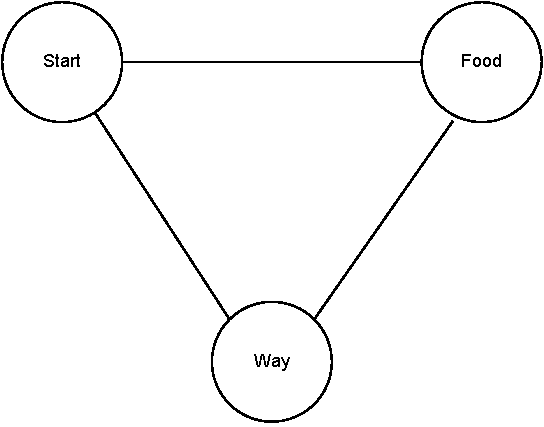
\includegraphics[scale=0.5]{figures/background/double_bridge_graph.pdf}}
		\caption{Model of the Double Bridge Experiment as a graph. The long branch consists of two edges (Start, Way), (Way, Food)}
		\label{fig:double_bridge_graph}
	\end{centering}
\end{figure}

Now $p_{is}(t)$ describes the probability that an ant at time $t$ at location $i$ chooses the short path $s$ and $p_{is}(t)$ the long path $l$. To define these probabilities, the pheromone level $\varphi_{ia}$ an ant encounters at node $i\in{(Start,Food)}$ on branch $a \in {(l, s)}$ has to be considered. The long branch $l$ is exactly two times longer than the short branch $s$ and therefore also takes two time-steps to traverse instead of one. This leads to the following equations:
$$p_{is}(t) = \frac{[\varphi_{is}(t)]^\alpha}{[\varphi_{is}(t)]^\alpha + [\varphi_{il}(t)]^\alpha}, \;p_{il}(t) = \frac{[\varphi_{il}(t)]^\alpha}{[\varphi_{is}(t)]^\alpha + [\varphi_{il}(t)]^\alpha},$$
where $p_{is}(t) + p_{il}(t) = 1$ and $\alpha$ is a parameter. The update of pheromones on the two branches is described as:
$$\varphi_{is}(t) = \varphi_{is}(t-1) + p_{is}(t-1)m_i(t-1) + p_{js}(t-1)m_j(t-1),$$
$$(i = Start, j = Food; i = Food, j = Start),$$
$$\varphi_{il}(t) = \varphi_{il}(t-1) + p_{il}(t-1)m_i(t-1) + p_{jl}(t-2)m_j(t-2),$$
$$(i = Start, j = Food; i = Food, j = Start),$$
where $m_i(t)$, the number of ants at node $i$ at time $t$ is given by:
$$m_i(t) =  p_{js}(t-1)m_j(t-1) + p_{jl}(t-2)m_j(t-2),$$
$$(i = Start, j = Food; i = Food, j = Start),$$
Dorigo and Stützle show in \cite{DBLP:books/daglib/0013523}, that simulations with $\alpha = 2$ lead to a quick convergence of the ants towards the use of the short branch.\\
To expand the described system, to find shortest paths in more complex graphs, requires the ants to additionally receive a small memory. This enables them to avoid loops and to remember the entire solution they built. They can then evaluate the built solution to determine the quantity of pheromone to deposit. As mentioned before, the performance can be greatly improved by adding evaporation to the pheromones.

\subsection{General Ant Colony Optimization}
To solve more general minimum cost problems on graphs ACO performs two main steps being the \textbf{solution construction} and the \textbf{evaluation}.\\
Firstly, a solution is constructed by an ant beginning at the starting node and incrementally adding neighboring nodes. The decision, which node to add next, is influenced by pheromones deposited in previous iterations. In the very first iteration the pheromone is uniformly distributed along the paths and the decision rule is therefore random. Additionally, a heuristic function $\eta$ can be used to find better results faster. A common heuristic for short paths is the inverse of the euclidean distance to the destination. Using a heuristic is a greedy approach and a balance between learning via pheromones and preset knowledge via heuristics is crucial. This procedure is repeated until the destination node is reached. Note, in case of grid planning a solution requires all nodes to be added. The order of how the nodes are added and over which edges is stored in memory.
The probability of an ant choosing path $i$ considering the heuristic can be formalized in the following way:
$$p_i = \frac{\varphi_i^\alpha\eta_i^\beta}{\sum_{j\in{w}}\varphi_j^\alpha\eta_j^\beta},$$
where $w$ is the set of all paths reachable from the current position and $i,j \in w$. $\varphi_i$ is the amount of pheromone on path $i$ and $\eta_i$ is the heuristic value on path $i$. $\alpha$ and $\beta$ are parameters to determine the relation of pheromones and heuristics in the decision of the ant. Furthermore, it holds $\sum_{k\in{w}}p_k = 1$. \\
Secondly, the build solution is evaluated and its cost is calculated. Now the amount of pheromone this particular solution should receive is set according to the cost. This could for example be the inverse of the solutions cost. Thereby, solutions with low cost receive more pheromones and vice versa. In the next iteration, the pheromone deposited from the previous solution influences the way in which new nodes are added. Pheromone evaporation can help to reduce the weight that older solutions have on the pheromone level where less information about the problem existed. Generally, more evaporation leads to more exploration of the search space. Evaporation also helps to bound the maximal amount of pheromone achievable. Update and evaporation can be formulated in the following way:
$$\varphi_i = (1-p)\varphi_i + p\Delta\varphi_i$$
$$\text{with } \Delta\varphi_i = \begin{cases}
	1 & \, \text{if i is part of solution}\\
	0 & \, \text{else}
\end{cases}$$
where $p$ is the evaporation factor and $\varphi_i$ is the amount of pheromone deposited on path i.
A detailed description of the presented ACO algorithm \textit{APMV} will be presented in section \ref{sec:antpowermv}.


\section{ACO In Grid Planning}

To bring ACO and grid planning together, one needs to formulate the grid planning problem in a way so it can be solved by an ACO algorithm. A suitable way to do this, is to use graphs as a model of the electric grid. Intuitively, the buses of the grid can be seen as nodes (sources, loads are transformers are directly coupled to the buses), whereas the transmission lines connecting the buses are the edges. Let $G = (B, E)$ be an undirected graph, where the nodes $B$ are the buses $b_1, b_2, ...$ of the grid and the edges $E$ resemble the transmission lines $t_1, t_2, ...$. The goal is to build a graph, where all nodes are connected at the lowest cost possible. Additional constraints like the topology of the graph also have to be considered. As long as the graph is well defined the ACO algorithm can operate in a similar way as previously shown.
The node which represents the transformer connecting the grid to the overlying HV level is used as a starting point. It serves as a source to the other buses electricity demand. At the start, none of the nodes are connected to each other and incrementally edges (transmission lines) are added to the graph until all nodes are connected through a path to the starting node (transformer). Afterwards, the cost of such a solution is calculated and the pheromone update is performed on the used paths accordingly.

\subsection{Delaunay Triangulation}\label{triangulation}
Theoretically, every network station could be connected with all other stations, which is infeasible in practice due to economic reasons. But also for computing, a reduction of the number of potential connections between network stations reduces the algorithms runtime exponentially (reduction of the search space). The Delaunay triangulation is a suitable method to reduce the number of potential lines between stations. It divides a surface with points into triangles by maximizing the minimum of all the angles of the triangles in the triangulation.
\begin{figure}[h]
	\begin{centering}
		{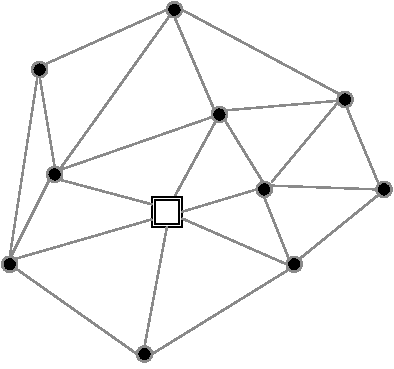
\includegraphics[scale=0.7]{figures/background/tri.pdf}}
		\caption{Delaunay Triangulation of a set of buses and a transformer.}
		\label{fig:tri}
	\end{centering}
\end{figure}
An example of this can be seen in Figure \ref{fig:tri}, where the transformer is marked with a square. Research shows, that for the related TSP only 1\% of the edges belong to the optimal solution and are not part of the triangulation \cite{schmitting2000traveling}. The exponential reduction of the number of connections between $N$ buses can be shown via the following equations:
$$e_{total} = \frac{1}{2}N(N-1)\text{ versus }e_{tri} = 3N - 3 - N_h$$
where $e_{total}$ is the number of all possible connections and $e_{tri}$ is the number of possible connections after applying the triangulation. $N_h$ is the number of nodes being part of the convex hull. \\

\subsection{Ant Graph}\label{ant_graph}
The triangulation can additionally be used to create a new graph called \textit{ant graph} which simplifies the mathematical formulation of the ring network planning problem \cite{rotering2013zielnetzplanung}. To build this graph, the incenter of the triangles and the transformer are taken as nodes (\textit{ant nodes}). Edges are created between triangles, which share a common side (\textit{ant edges}). Since every triangle already constitutes a ring in itself using them to built a solution which satisfies the topological constraints is very helpful. If a neighboring ant node (triangle) is added, the hull of the represented triangles again forms a ring. As long as this ring contains the transformer as a node a valid ring network design is produced. An example is shown in Figure \ref{fig:aco_grid}, where the unfilled circles represent the \textit{ant nodes} and the dotted lines the \textit{ant path}.

\begin{figure}[h]
	\begin{centering}
		{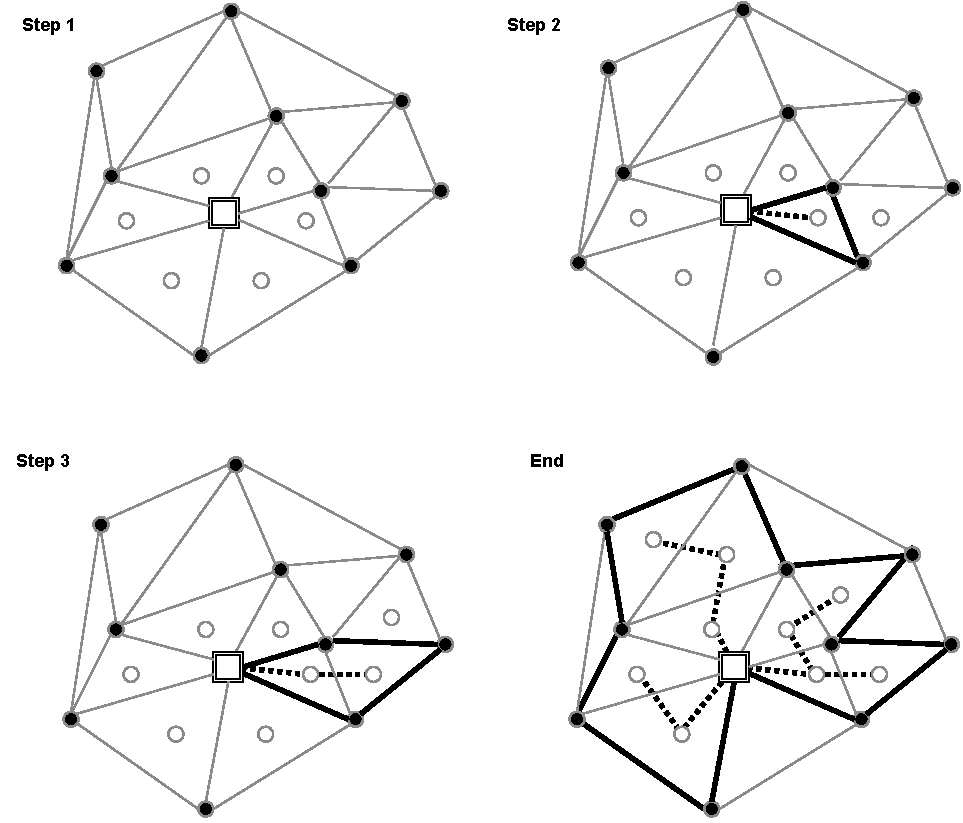
\includegraphics[width=\textwidth]{figures/background/aco_grid.pdf}}
		\caption{Building a solution on the ant graph.}
		\label{fig:aco_grid}
	\end{centering}
\end{figure}

The expansion is started at the transformer (square). In step 1 no \textit{ant nodes} are added to the transformer. The first expansion options are its neighboring \textit{ant nodes}. After the first node is added in step 2, a new expansion option is accessed. The two stations (filled circles) together with the transformer already represent a valid ring network structure. In step 3 a second triangle is added, so the hull of the two triangles is the new intermediate ring network solution. This procedure is repeated until all stations are covered by triangles represented by ant nodes.

\subsection{Switches}
When a ring is finished, an open switch is placed at a bus to determine the separation point of the ring. The buses before and after the switch are supplied with power from their respective part of the ring. Only in case of a failure, the switch is closed such that cut off buses are reconnected to the power supply. Thereby, the \textit{n-1 criterion} of MV grids can be fulfilled. Usually, the switch is placed at a position in the ring, where the load of both parts of the ring are balanced.






    \chapter{Approach}\label{chap:approach}
First the problem definition is formulated, followed by the presentation of the ACO algorithm \textit{APMV} for solving it.

\section{Optimization Problem}\label{optiproblem}
The goal of the ACO algorithm in grid planning is to connect the loads and generators of the grid in the most cost effective way whilst satisfying the side constraints. The topological side constraint is the \textit{n-1 criterion}, which requires every bus to be reachable via at least one alternative route. This resembles a ring structure in the graph (multiple rings are also possible). As described in \ref{ant_graph}, this can be done via finding the spanning tree of the \textit{ant graph} which results in the lowest cost of its hull. The process of building the spanning tree can already stopped, if all stations of the network are covered. There already exist several algorithms, like Boruvkas algorithm, which can find a minimum spanning tree in polynomial time ($O(mlogn)$, where $m$ is the number of edges and $n$ the number of vertices). Unfortunately, the here formulated problem differs from the simple minimum spanning tree problem because not the cost of the \textit{ant edges} but the cost of the hull of the spanning tree has to be minimized. Trying to deduce the cost of the \textit{ant edges} from the cost of the hull is impossible since the edge weight depends on the node from which the edge is expanded. This can be illustrated in Figure \ref{fig:different_cost}.
\begin{figure}[h]
	\begin{centering}
		{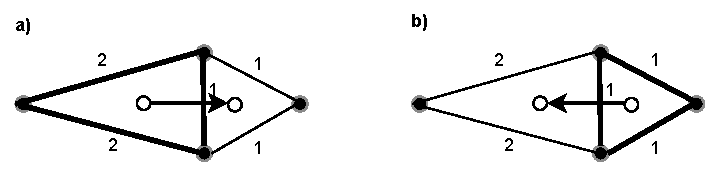
\includegraphics[scale=0.9]{figures/approach/different_cost.pdf}}
		\caption[Cost of ant edge]{The cost of an ant edge depends on the node from which it is getting expanded from.}
		\label{fig:different_cost}
	\end{centering}
\end{figure}
 \\
The left triangle has a cost of five, the right triangle a cost of three and their hulls when combined a cost of six. If the edge starts at the incenter of the left triangle and expands the right triangle additional cost of one are added to the hull ($5+3-2$, since the shared side of the triangles needs to be subtracted). Therefore, one could assign cost of one to the edge. But in the reverse case, the left triangle adds three to the cost of the hull ($3+5-2$).

Additionally for the problem formulation, two electric side constraints need to be fulfilled. The maximum capacity of the power flow on a transmission line must never be exceeded. Similarly, the voltage violation limits of buses in the network must be complied with. In the case of MV grids in Germany according to DIN EN 50160, the voltage deviation at any bus at any time must not exceed a limit of  $\pm$ 5\%. The power that flows through a line segment shall never be more than 50\% of the lines maximum capacity. The voltages and power flows in the network can be calculated via a power flow analysis (PFA).

%According to DIN EN 50160, under normal operating conditions, 95\% of the 10-minute average of the measured RMS value of each weekly interval must be within the limits of ±10\% of the nominal voltage.

%As inputs, PFA requires the impedances of lines and transformers, the voltages at sources, and the powers at sources, loads, and transformers
%TODO: check for exact electrical side constraint!

\section{Ant-Power-Medium-Voltage}\label{sec:antpowermv}
The algorithm \textit{APMV} was developed to solve the optimization problem formulated in the previous section. It is an advancement of the algorithm presented by Zeller in \cite{zeller2021planung} and uses concepts presented by Dorigo et. al. and Rotering.


\subsection{Input and Parameters}\label{parameters}
The algorithm was specifically designed for the medium voltage level. If the input is a mixed grid and consists of multiple voltage levels, the medium voltage part needs to be extracted first (see \ref{sec:extraction}). As a data format the algorithm accepts a \textit{PyPSA}-network (see \ref{pypsa}) as an input file.\\
Important Parameters to set are the following:
\begin{itemize}
	\setlength\itemsep{-0.8em}
	\item \textbf{lineType}: Specifies the type of the line which should be build. This determines the lines resistance, reactance and capacity of its maximal power flow.
	\item \textbf{antsPerColony}: How many ants are building a solution in every iteration.
	\item {\boldmath{$q0$}: Probability that the ant chooses the best option (according to pheromone level + heuristic).
	\item \textbf{$\alpha$}: Parameter to determine the influence of the pheromones in the expansion decision.
	\item \textbf{$\beta$}: Parameter to determine the influence of the heuristic value in the expansion decision.
	\item \textbf{$\rho$}: Parameter for the global pheromone update. Determines how much pheromone is deposited to reward the best solution.
	\item \textbf{$\xi$}: For the local pheromone update. Determines how much pheromone is removed from already used paths to evoke more exploration.}
	\item \textbf{iterations}: Number of iterations of the algorithm.
	\item \textbf{maximalRingsize}: Maximal number of buses allowed per ring.
\end{itemize}


\subsection{APMV Implementation}
In algorithm \ref{alg:high_level} the high-level implementation of \textit{APMV} is shown. At the very beginning, the input grid is prepared to be compatible with the algorithm in a preprocessing step. Afterwards the initial pheromone is deposited. As already explained in Chapter \ref{ACO}, every ant in the algorithm builds one solution per iteration. Out of these solutions the best one is kept and rewarded with pheromones which influences the solution building process of the next iteration ($globalPheromoneUpdate()$). After a postprocessing step, the overall best solution and its cost is returned. $\varphi_0$ is the pheromone distribution at the start and $N$ is the number of stations in the network.

\begin{algorithm}[h]
	\caption{High-level implementation of \textit{APMV}}
	\label{alg:high_level}
	\begin{algorithmic}[1]
		% \ttfamily
		\State $preprocessing$(grid) \alignedComment{extraction of MV grid and triangulation}
		\State $\varphi_0 \gets initializePheromones()$ \alignedComment{$\frac{1}{N}$, with $N$ = number of stations}
		\State lowestCostSoFar $\gets \infty$ 
		\ForEach{i $\in$ iterations}
		\State $solutionsPerIteration \gets \emptyset$
		\ForEach{ant $\in$ antsPerColony}
		\State solution $\gets createSolution(\varphi_i)$
		\State solutionsPerIteration $\gets$ solutionsPerIteration $\cup$ solution
		\EndFor
		\State bestSolutionIter $\gets argmin$($cost$(), solutionsPerIteration)
		\If{$cost$(bestSolutionIter) < lowestCostSoFar}
		\State lowestCostSoFar $\gets cost$(bestSolutionIter)
		\State bestSolution $\gets$ bestSolutionIter
		\EndIf
		\State $\varphi_i \gets globalPheromoneUpdate$($\varphi_{i-1}$, bestSolution)
		\EndFor
		\State $postprocessing$(bestSolution) \alignedComment{export back into \textit{PyPSA} format}
		\State \Return bestSolution, lowestCostSoFar
	\end{algorithmic}
\end{algorithm}

\subsubsection{Global Pheromone Update}
The function \textit{globalPheromoneUpdate()} is performed once after each iteration and deposits additional pheromones on the nodes expanded by the best solution found so far. Over time this enables the algorithms to learn from previous iterations and shows which nodes generally lead to good or bad solutions. The formula for the global pheromone update on all visited nodes $i$ of the best solution is the following:
$$\varphi_i = (1-\rho) \varphi_i + \rho \frac{c_{est}}{c_{best}},$$
where $\rho \in (0,1)$, $c_{best}$ are the cost of the best solution found so far and $c_{est}$ are the estimated cost of the solution. The reciprocal of the $c_{best}$ is is used such that low cost are rewarded by high amounts of pheromone. It is normalized by the $c_{est}$ to better reflect the quality of the solution. As long as $\frac{c_{est}}{c_{best}} > \varphi_i$ the pheromone increases. Otherwise, the pheromone level can also decrease.
%amount = estimated_min_expansion_cost / min_cost
%pheromone_i = pheromone_i * (1-rho) + amount * rho

\subsection{Solution Creation of Ants}
In algorithm \ref{alg:solution} the schematic implementation of the $createSolution()$ function is shown. The expanded nodes are ant nodes and the $solution()$ method checks whether the hull of the set expandedNodes covers all stations. The $expand()$ method finds the next node which should be added and depends on the pheromones $\varphi$, the heuristic $\eta$ and the neighborhood $neighbor()$ of the already expanded nodes. In the $localPheromoneUpdate()$, the pheromone gets decreased on the already used path to increase exploration and reduce the chance of convergence towards a local minimum. When $solution$(expandedNodes) is true, a solution is found and is returned with the updated pheromone level $\varphi$. 
\begin{algorithm}[h]
	\caption{Implementation of createSolution($\varphi$)}
	\label{alg:solution}
	\begin{algorithmic}[1]
		% \ttfamily
		\State expandedNodes $\gets \emptyset$
		\While{$solution$(expandedNodes) $=$ false}
		\State newNode $\gets$ $expand(\varphi, \eta, neighbor$(expandedNodes)
		\State expandedNodes $\gets$ expandedNodes $\cup$ $expand(\varphi, \eta, neighbor$(expandedNodes))
		\State $\varphi \gets$ $localPheromoneUpdate$(newNode, $\varphi$)
		\EndWhile
		\State \Return expandedNodes, $\varphi$
	\end{algorithmic}
\end{algorithm}

\subsubsection{Local Pheromone Update}
The function \textit{localPheromoneUpdate()} is executed every time the ant expands a new node and generally reduces the amount of pheromone on that node. This should increase the chance of other ants to use different paths instead and therefore increase exploration. The pheromone level of node $i$ gets updated via the following rule:

$$\varphi_i = (1-\xi)\varphi_i + \xi \varphi_{init},$$
where the parameter $\xi$ determines, how much the pheromone level should revert back to the initial pheromone level $\varphi_{init}$. 
%self._triangulation.get_shallow_copy_graph().edges[edge]['pheromone'] = \
%self._triangulation.get_shallow_copy_graph().edges[edge]['pheromone'] * (1 - self._xi) + \
%self._xi * self._initial_pheromone
\subsubsection{Heuristic}
The purpose of the heuristic $\eta$ is to provide additional guidance for the ant when making the decision which node to expand next. Especially in earlier iterations when the algorithm has not learned much yet (via pheromones) the heuristic can lead to better quality solutions. The overall cost of a built solution is roughly proportional to the length of the rings. The aim is to estimate the additional cost of expanding a node, so the ant can chose the one with the lowest cost. When adding a node (which represents a triangle) the length of the ring increases by the perimeter of the triangle minus two times the shared side (see Figure \ref{fig:heuristic} a)).
\begin{figure}[h]
	\begin{centering}
		{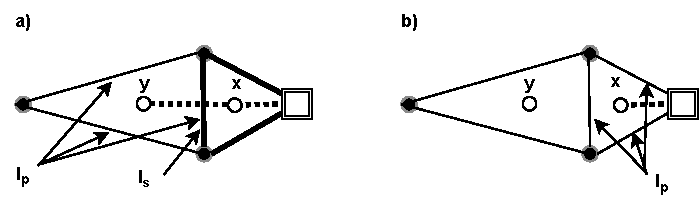
\includegraphics[scale=0.9]{figures/approach/heuristic.pdf}}
		\caption{Calculating the heuristic value.}
		\label{fig:heuristic}
	\end{centering}
\end{figure}
 \\
The reciprocal of the length a triangle (ant node) adds to the ring is used as a heuristic.
$$\eta_{x,y} = \frac{1}{l_{p} - 2l_{s}}$$
As explained in \ref{optiproblem} this heuristic not only depends on the expanded node $y$, but also on the node from which it gets expanded $x$. This leads to high heuristic values for triangles with short sides and low heuristic values for triangles with long sides. For the first triangle that gets expanded from the transformer node, the heuristic value is just the sum of the length of all sides, since there is no shared side (see Figure \ref{fig:heuristic}) b). The problem with this (greedy) heuristic is that it does only minimizes the next expansion step and not the length of the ring at the end. Additionally, it does not account for the cost of voltage violations on buses.

\subsubsection{Expansion rule}
As shown in algorithm \ref{alg:solution}, the $expand()$ method depends on the heuristic $\eta$, the pheromones $\varphi$ and is limited to the neighbors of the already expanded ant nodes. As suggested by ACS \cite{ant_coloy_system}, the next node $s \in neighbor(x)$, with $x$ being the already expanded nodes and $s_i \in neighbor(x)$, is chosen according to the following rule:
$$p_s = \begin{cases}
	argmax_{s_i}(\varphi_{s_i}^\alpha \eta_{s_i}^\beta) & \, \text{, if q $\leq$} q_0\\
	\frac{\varphi_s^\alpha\eta_s^\beta}{\sum_{s_i}\varphi_{s_i}^\alpha\eta_{s_i}^\beta} & \, \text{, if q >} q_0
\end{cases}$$

where $q \in [0,1]$ is a uniformly distributed random variable. If the value of $q$ is greater than the threshold $q_0$ the algorithm choses the best known path (exploitation) and if $q$ is lower than $q_0$ the algorithm choses randomly (exploration). 

\subsection{Switches}
$APMV$ places the switches exactly in the middle of the ring (regarding the number of stations). This is done regardless of load or generation of its buses. Most of the time, this leads to fairly balanced loads on both parts of the ring. In future work however, switches could be placed based on the load and generation distribution inside the ring to ensure a good balance.

\subsection{Cost function}
The cost function plays a crucial part in the algorithm since it determines the pheromone distribution of the next iteration and therefore how the algorithm improves. The costs consist of two parts, the cost of building lines $b(x)$ and a penalty term for violations of electrical constraints $e(x)$.
$$cost(x) = b(d(x), c(x)) + e(x),$$
where $x$ is the network of the solution, $d(x)$ are the digging cost and $c(x)$ are the cable cost. The building cost and the penalty term will now be discussed in further detail.

\subsubsection{Building cost}
Concerning the cost of building lines, there are the acquisition costs of new transmission cables and the digging costs of laying the cables into the ground. As an estimation for standard MV lines are taken cable cost of 130K Euro/km and digging cost of 100K Euro/km. These values of course fluctuate over time and have to be adapted for the specific situation. If the algorithm suggests building a line between two buses, where a line already exists, the costs are set to zero (assuming they can still be used in the future). For new transmission lines, the algorithms tries to predict the length and where the cable is laid along via the street network. Usually, cables are laid next to streets for better access and less invasive construction works. This is taken into account by using a tool developed by John \cite{robert_john}, which uses data from open street map to find the distance and the path between two network stations alongside streets. John first creates a graph from open street map in a given area, connects the network stations to it and then calculates the shortest path between the stations using Dijkstra. If the distance between two stations cannot be estimated via open street map, the straight distance calculated via the haversine formula multiplied by $1.2$ is used.

\subsubsection{Penalty term}
The second part of the costs is a penalty term accounting for voltage violations of buses and loading violations of lines of the target grid. Therefore, a PFA is conducted, which calculates the voltages at all buses and the power flowing in each line of the network. If values exceed their limits penalties are added to the cost. These penalty costs are orders of magnitude greater in comparison to the building costs. Thereby, the ants get rewarded much more by finding solutions without load flow violations. With enough iterations this practically guarantees that a convergence towards a solution has either no load flow violations at all or it is impossible to find a solution without it.

%TODO: check load flow analysis again!
%voltage deviations for buses
%loading violations for lines

\subsection{The Back-and-Forth Case}\label{backandforth}
As Zeller already points out in \cite{zeller2021planung}, there exist cases in which the standard process of building the hull  of the \textit{ant graph} as described by Rotering does not work. Such a case is shown in Figure \ref{fig:backandforth}.
\begin{figure}[h]
	\begin{centering}
		{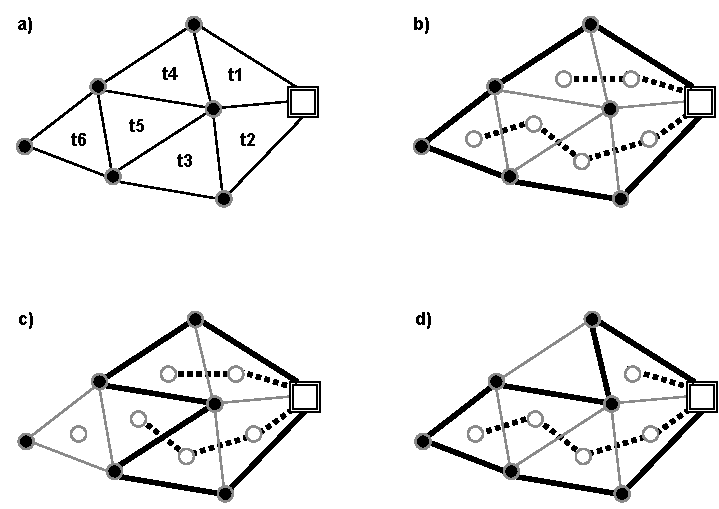
\includegraphics[scale=0.9]{figures/approach/backandforth.pdf}}
		\caption[Problematic case of building a ring]{Problematic case of building a ring via the hull of the ant graph.}
		\label{fig:backandforth}
	\end{centering}
\end{figure}
If the expansion of ant nodes proceeds as shown in case b), one station is not contained in the hull. The problem here is that it is possible to expand a triangle where all its three stations are already covered by the hull at that point in time (t5 in c)). This is necessary though because the triangle t6 is only reachable via t5. Zeller's approach is to allow the expansion of the crucial triangle t5 anyways, but to do the routing in a way so it maintains the ring structure and it does not lose the connection to the node in the middle (Zeller called this a \textit{back-and-forth} case). Unfortunately, his solution only worked in this specific case and did not cover further problems caused by the same issue. \textit{Back-and-forth} cases can be chained indefinitely and Zeller only solved them until a certain depth. Another possible attempt of solving this issue would be to create two parallel lines from the hull to the unconnected station in the middle. This would maintain the ring structure but also connect the outer station twice. Therefore, \textit{APMV} prohibits the expansion to triangles where all their three stations are already covered. If such a case occurs, the ant is getting restarted and a different solution is constructed (d). Depending on how often the ant needs to get restarted the performance of the algorithm reduces. During the creation of this work it was not clear how often such cases would appear in real networks and if it would be worth to develop an exact mechanism, which covers all problematic cases. For the real network example evaluated in this work however, a run of 1000 iterations and 15 ants per iteration only required 40 ants to be restarted, which does not represent a major issue ($\frac{40}{15000} = 0.00226 \%$). I leave for future work to find a method for an exact solutions to this problem.

\subsection{Multiple Rings}
To increase security it is common to limit the amounts of stations per ring to a certain maximum. Therefore, it is possible that multiple rings are required to cover all stations in the network. Another reason might be that rings connecting to different HV/MV transformers overlap in certain parts. Although it is possible to have multiple lines on the same path, the buses must only be connected to exactly one ring. To avoid the connection of buses to multiple rings it would be possible to check during the solution creation whether a bus is already covered by a different ring and to forbid its expansion. This however could lead to many dead ends, since the algorithm is limited to the expansion to neighboring nodes created by the triangulation. Therefore, \textit{APMV} allows the rings to expand to every neighbor independent of their potential connection to a different ring and to resolve the issue in a postprocessing step.\begin{figure}[h]
	\begin{centering}
		{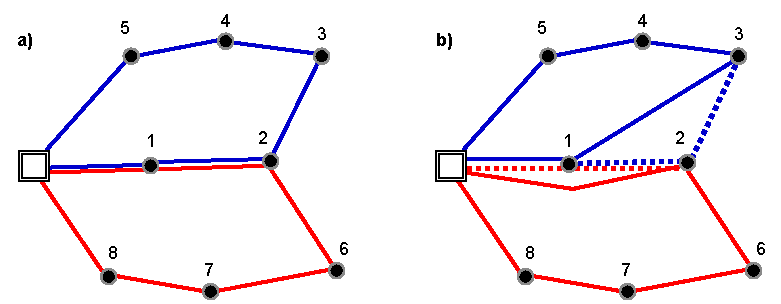
\includegraphics[scale=1]{figures/approach/busnosplit.pdf}}
		\caption{Handling of overlapping rings.}
		\label{fig:busnosplit}
	\end{centering}
\end{figure}
Figure \ref{fig:busnosplit} a) shows a case where two rings (blue and red) are partly overlapping at buses 1 and 2. To resolve the issue bus 1 gets chosen to be connected to the blue ring and bus 2 to the red ring. The connections of buses to lines are depicted by the continues lines and how the cables are put into the ground is illustrated by the dotted line. The lines basically stay where they should be according to the triangulation but the buses are just connected to maximal one line. \textit{APMV} determines the allocation of buses to rings randomly. In future work this could be based on balancing the load and generation of rings.

\subsection{Ring Size and Triangulation}\label{sec:tri_problem}
Limiting the number of stations can be done easily during the expansion process of the ant. When an ant expands a new triangle during the solution building process, the number of stations of the ring also increases by one (neighboring triangles already share two corners). This applies to all triangles except the very first one expanded from the HV/MV transformer, where two stations are added. The number of stations per ring is therefore the number of expanded triangles incremented by one. When the ant reaches the maximum number of triangles it is allowed to expand, it stops with the expansion and starts constructing a new ring starting from the HV/MV trafo. Downwards, the maximal number of stations per ring is limited depending on the structure of the grid. \\
When the maximal number of stations per ring is limited, another complication in conjunction with the triangulation can arise. Namely, the number of neighboring triangles of the transformer is limiting the number of rings which can be built.
\begin{figure}[h]
	\begin{centering}
		{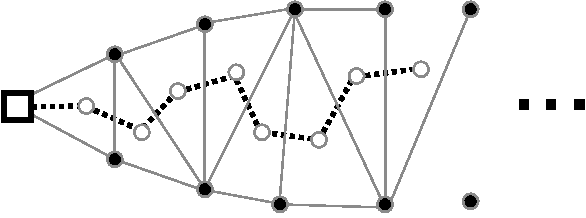
\includegraphics[scale=0.9]{figures/approach/trifail.pdf}}
		\caption[Limited ring size]{Limitations of triangulation and limited ring size.}
		\label{fig:trifail}
	\end{centering}
\end{figure}
A worst case scenario is depicted in Figure \ref{fig:trifail}. There can exist an arbitrary number of stations in the network but through the triangulation only one neighboring triangle to the transformer is built. After the first ring reaches its maximal number of stations, there is no triangle left for another ring to start its construction. To counteract this bottleneck, the expansion rule described in \ref{backandforth} is relaxed for neighboring triangles of the transformer. This means that it is allowed to expand a triangle even though all three of its stations are already covered. In general this technique helps to find more solutions, although in the shown example it also would not work, since there only exist one available expansion option for each triangle. Another possible fix, is to increase the maximal number of allowed stations per ring. Similar to \ref{backandforth}, \textit{APMV} just tries to restart the solution building process in the hope to find a different expansion order, which does not result in a restart. For the real network evaluated in this work, the number of restarts out of 1500 attempts in relation to the maximal ring size is depicted in Figure \ref{fig:restarts}. For a maximal ring size of 7, every solution building attempt has to be restarted, so no solution could be found. Manual verification confirms that it is impossible to create a solution with only 7 stations per ring. In practice however manual verification is too time consuming, therefore sufficiently many iterations and ants per iteration have to be chosen. For 8 or more rings valid solutions are found by the algorithm. When the ring size is unlimited, almost all attempts lead to valid solutions. For critical ring sizes though runtime can be compromised considerably.
\begin{figure}[h]
	\begin{centering}
		{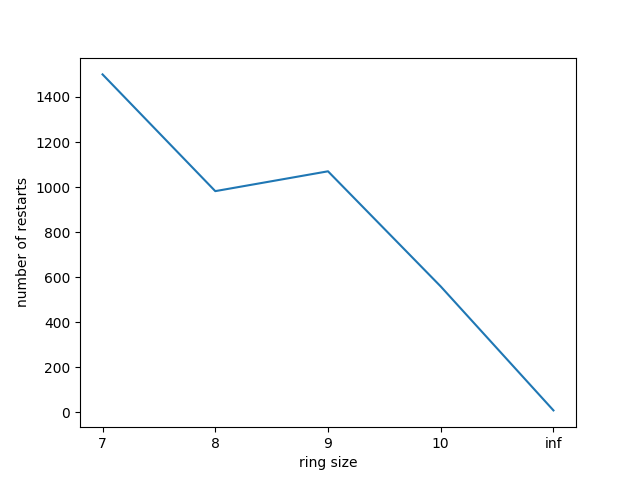
\includegraphics[scale=0.6]{figures/approach/restarts.png}}
		\caption[Number of restarts]{Number of restarts for different maximal ring sizes.}
		\label{fig:restarts}
	\end{centering}
\end{figure}


The approach of \textit{APMV} is to prevent the expansion of critical triangles which could lead to faulty network structures already during the solution building process. The reason not to fix an invalid solution in a postprocessing step is that it seems more practical. Without preventing the expansion of certain triangles, it is impossible to trace back and classify the exact reasons for a failed solution building attempt in hindsight. And without this classification of errors a corresponding "reparation" is very difficult. For future work, it might be an interesting task to find a postprocessing procedure which fixes invalid solutions created with an unrestricted expand method. This would prevent the need for restarting the solution building process and could therefore speedup the algorithms runtime.

\subsection{Run Time}
The time complexity of the algorithm mainly depends on the number of constructed solutions $n_{col} n_{ants} n_{iter}$ and the size of the network, where $n_{col}$ is the number of colonies, $n_{ants}$ is the number of ants and $n_{iter}$ is the number of iterations. Every constructed solution performs a PFA which has a time complexity of $O(B^3)$ in the worst-case, with $B$ being the number of buses. Additionally, every solution must expand nodes until all nodes are covered. This could take up to $B$ expansion steps. In the decision process the ant needs to consider up to $B$ possibilities which bus to expand next. This leads to $O(B^2)$ steps in the worst-case. In total this sums up to a runtime of $O(n_{col} n_{ants} n_{iter} (B^3+B^2))$. However, depending on the structure of the grid and the input parameters an arbitrary number of restarts of the ant could slow down the algorithm indefinitely.





    \chapter{Experiments}\label{chap:experiments}

\section{Settings}
\subsection{Libraries}\label{pypsa}
A key role for the implementation plays \textit{PyPSA} (Python for Power System Analysis) \cite{brown2017pypsa}, which is a toolbox to simulate and optimize power systems. The components of its network container are very closely related to the network components presented in section \ref{sec:components}. \textit{PyPSA's} Buses are the fundamental nodes to which all loads, generators, lines and transformers attach. According to Kirchhoff's current law everything feeding in out of the buses is balanced out to enforce energy conservation. The data is stored in \textit{pandas} DataFrames to enable efficient calculations. \textit{PyPSA} is also able to perform a power flow analysis on the network, which is important for the calculation of the penalty term among other functionalities. \textit{Networkx} is used by the algorithm to store and modify the graph which represents the electric grid.

\subsection{Example Grid}
For testing and evaluating the algorithm the grid of a village in rural Germany is used (exact name and location is omitted due to data protection). It is a mixed grid which consists of a medium and low voltage level. It connects to the higher voltage level from the south (cut off). It consists of 1857 buses, 1851 lines, 16 MV/LV transformer stations which connect the medium voltage level to the underlying low voltage level and 1 HV/MV transformer which connects the whole network to the upstream high voltage grid. \\
Although the network contains only 17 transformers, the number of possible rings, which connect the transformers is very large ($\frac{17!}{2} \approx 1.77*10^{14}$ [number of permutations divided by two, since the exact reverse order of stations is considered the same ring]). \\
\begin{figure}[h]
	\begin{centering}
		{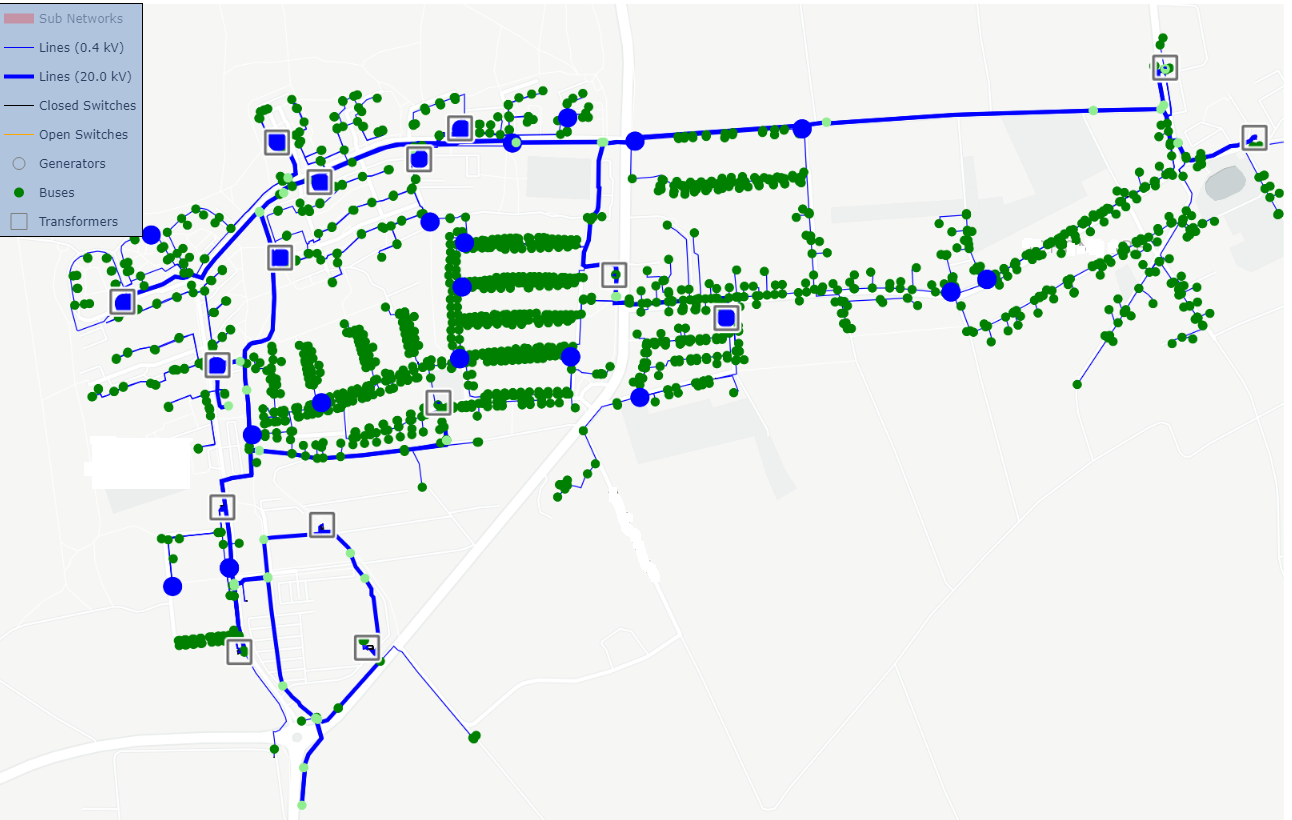
\includegraphics[scale=0.5]{figures/experiments/enwg_mixed.png}}
		\caption{The grid used for testing. (internally developed tool used for visualization)}
		\label{fig:enwg_mixed}
	\end{centering}
\end{figure}

\subsection{Grid Extraction}\label{sec:extraction}
The algorithm was specifically designed for the medium voltage level and therefore the input grid needs to fulfill the following requirements:
\begin{itemize}
	\setlength\itemsep{-1em}
	\item The input grid should contain only medium voltage buses (20 kV)
	\item All buses must have coordinates (for the triangulation)
	\item The buses loads are an aggregation of the loads of the underlying LV grid.
	\item The input grid only contains MV transmission lines (20 kV)
	\item The lines always directly connect two buses. 
	\item There has to exist at least one HV/MV transformer from where the algorithm can start.
\end{itemize}

\begin{figure}[h]
	\begin{centering}
		{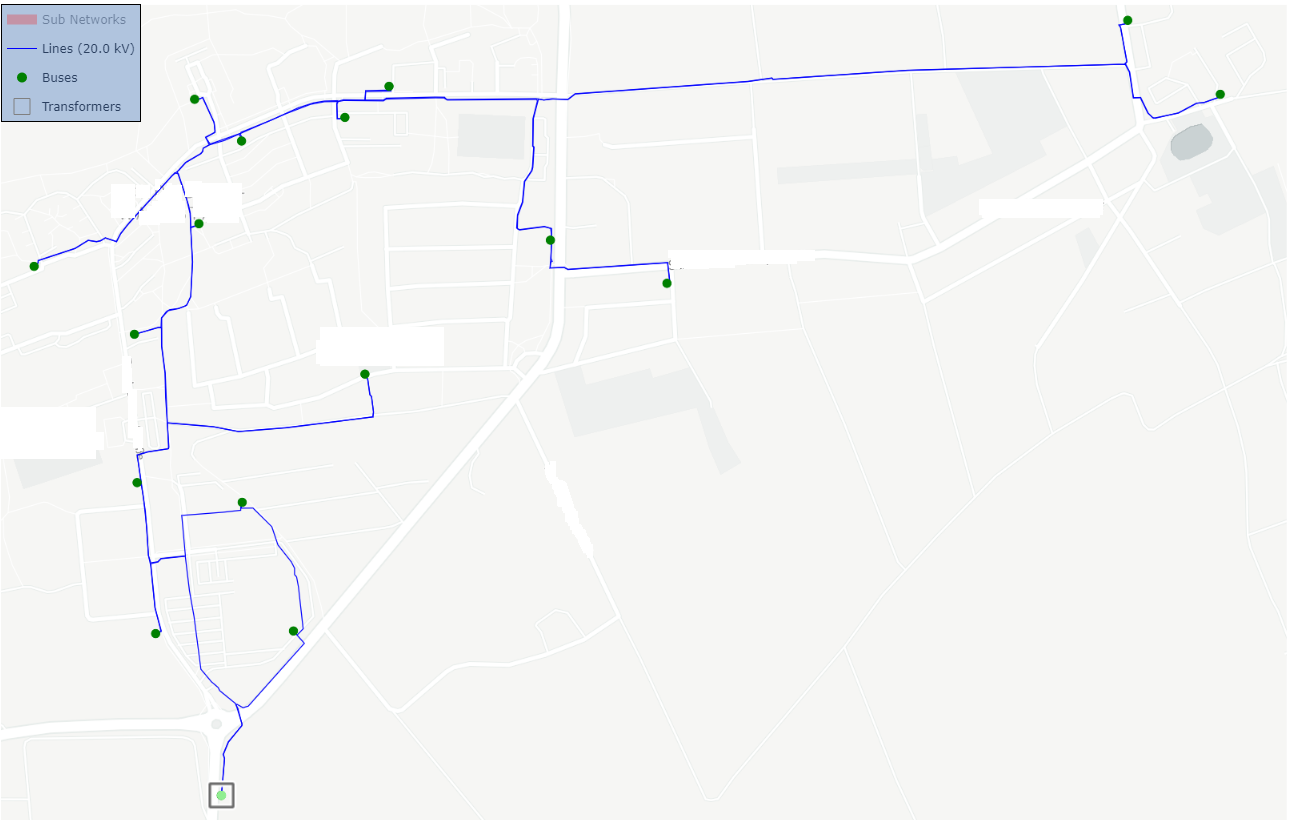
\includegraphics[scale=0.5]{figures/experiments/enwg_mv.png}}
		\caption{Middle voltage part of the grid.}
		\label{fig:enwg_mv}
	\end{centering}
\end{figure}


In a preprocessing step the MV part of the original grid is extracted (see Figure \ref{fig:enwg_mv}), to bring the input of the algorithm in the required form. After the extraction only the MV buses of the transformers are kept (in \textit{PyPSA} transformers connect two buses of different voltages). The task of the algorithm is to connect the buses via transmission lines in the most cost effective way, while satisfying the given side constraints. The blue lines are MV cables which already exist in the network and which can be used by the algorithm at zero cost. The green dots resemble the buses.



\begin{figure}[h]
	\begin{centering}
		{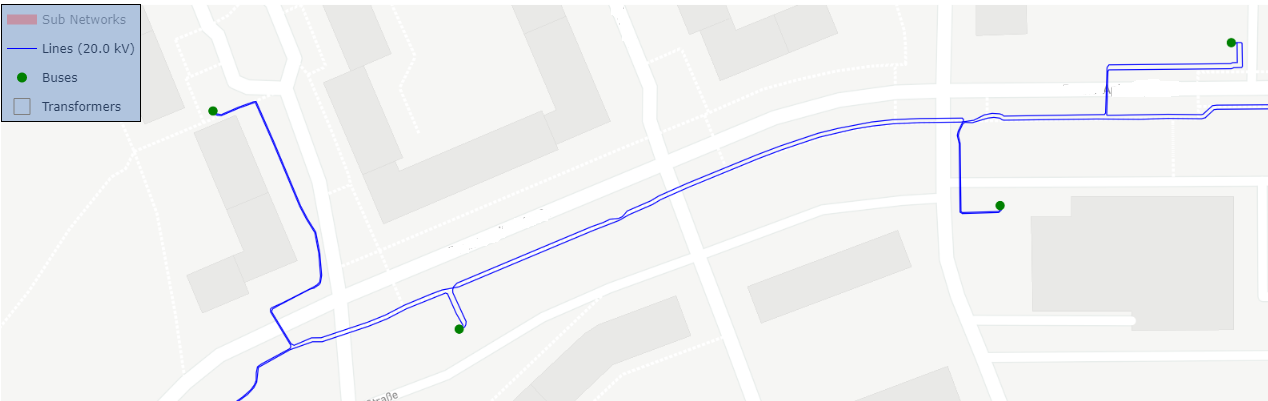
\includegraphics[scale=0.5]{figures/experiments/enwg_zoom.png}}
		\caption[Example graph zoom]{Parallel lines in the ring of the MV grid.}
		\label{fig:enwg_zoom}
	\end{centering}
\end{figure}

At first glance, the topology of the extracted MV grid does not look like it possesses the required ring structure. Only when zoomed in it is possible to see, that through parallel lines, the ring structure is maintained (see Figure \ref{fig:enwg_zoom}). It is debatable however, whether is it useful to put two lines in parallel to achieve adequate security. More to this in the discussion section \ref{sec:discussion}.


%\begin{figure}[h]
	\begin{centering}
		{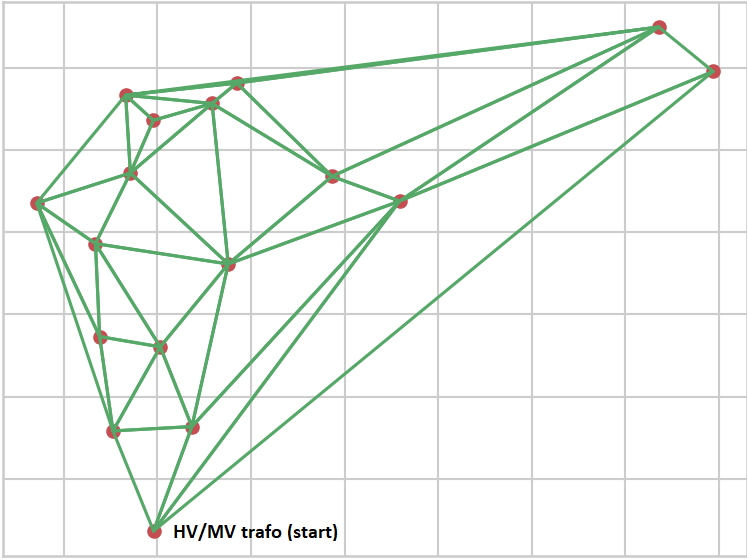
\includegraphics[scale=0.5]{figures/experiments/1000_iter/tri_1000.png}}
		\caption{Triangulation of the MV grid.}
		\label{fig:tri_1000}
	\end{centering}
\end{figure}


\begin{figure}
	\centering
	\begin{minipage}{.5\textwidth}
		\centering
		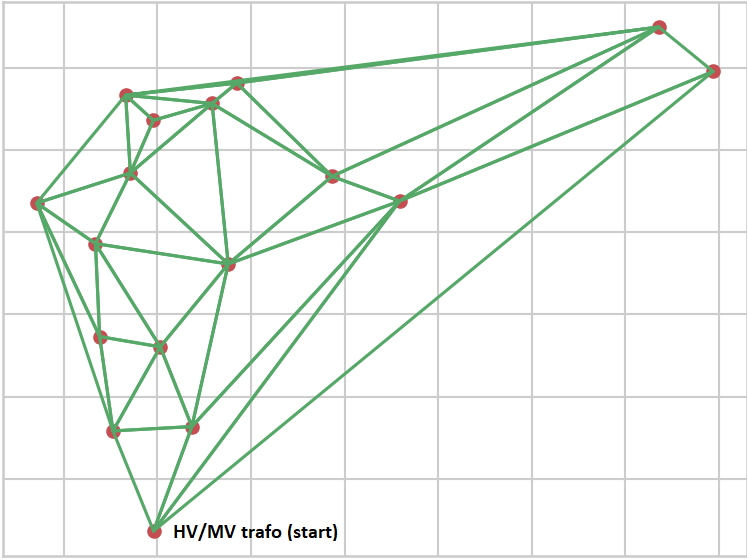
\includegraphics[width=.9\linewidth]{figures/experiments/1000_iter/tri_1000.png}
		\captionof{figure}{Triangulation.}
		\label{fig:tri_1000}
	\end{minipage}%
	\begin{minipage}{.5\textwidth}
		\centering
		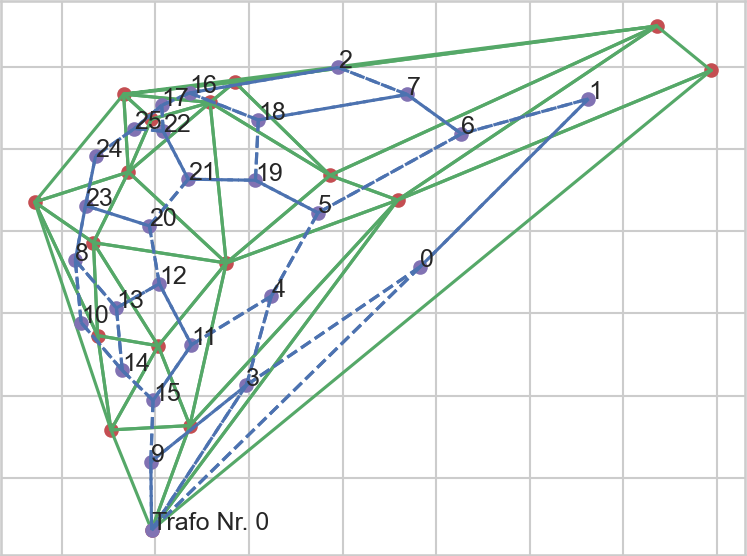
\includegraphics[width=.9\linewidth]{figures/experiments/1000_iter/tri_ant_1000.png}
		\captionof{figure}{Ant graph.}
		\label{fig:tri_ant_1000}
	\end{minipage}
\end{figure}

 %(green) and ant graph (blue) of the MV grid.
In Figure \ref{fig:tri_1000} the triangulation of the buses of the MV grid is shown in a schematic view. From the triangulation, the ant graph is built. Figure \ref{fig:tri_ant_1000} shows the associated ant graph. The blue ant nodes are the incenter of the triangles. Neighboring ant nodes are connected via an edge (dotted lines do not have a specific meaning in this context).

%\begin{figure}[h]
	\begin{centering}
		{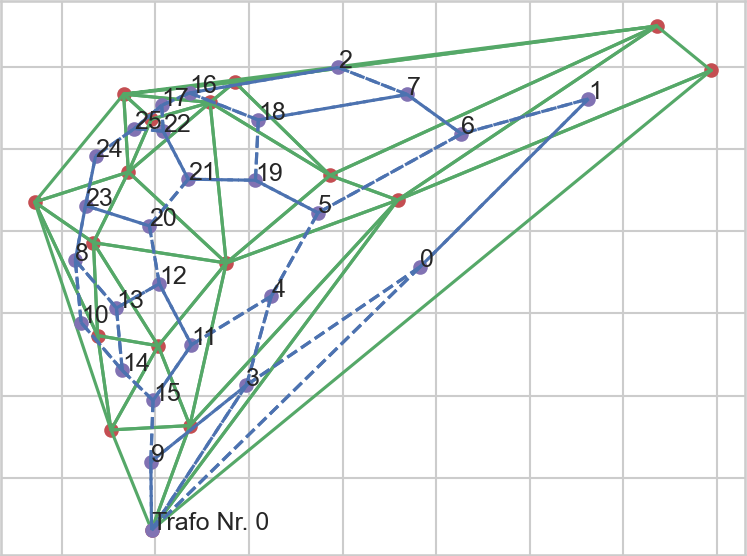
\includegraphics[scale=0.5]{figures/experiments/1000_iter/tri_ant_1000.png}}
		\caption{Triangulation (green) and ant graph (blue) of the MV grid.}
		\label{fig:tri_ant_1000}
	\end{centering}
\end{figure}


\section{Results}

\begin{figure}[h]
	\begin{centering}
		{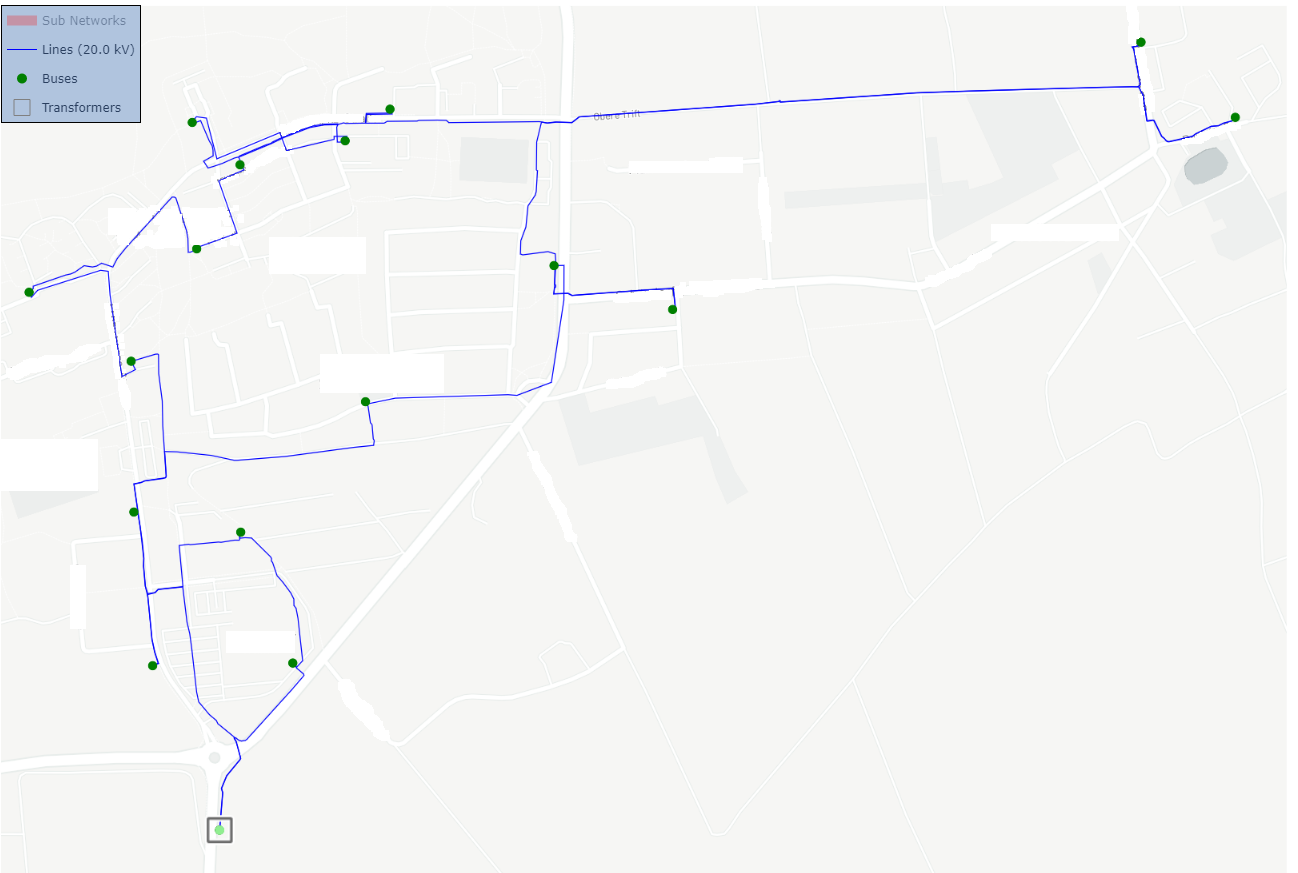
\includegraphics[scale=0.5]{figures/experiments/1000_iter/pypsa_1000.png}}
		\caption{Result network of best found MV grid.}
		\label{fig:pypsa_1000}
	\end{centering}
\end{figure}


The best result found by APMV is shown in Figure \ref{fig:pypsa_1000}. Most of the lines which are used in the input grid are also part of the result grid since they can be reused at zero cost. Four lines are new and added by the algorithm alongside streets. The penalty term for electric constraint violation is kept to zero.

\begin{figure}[h]
	\begin{centering}
		{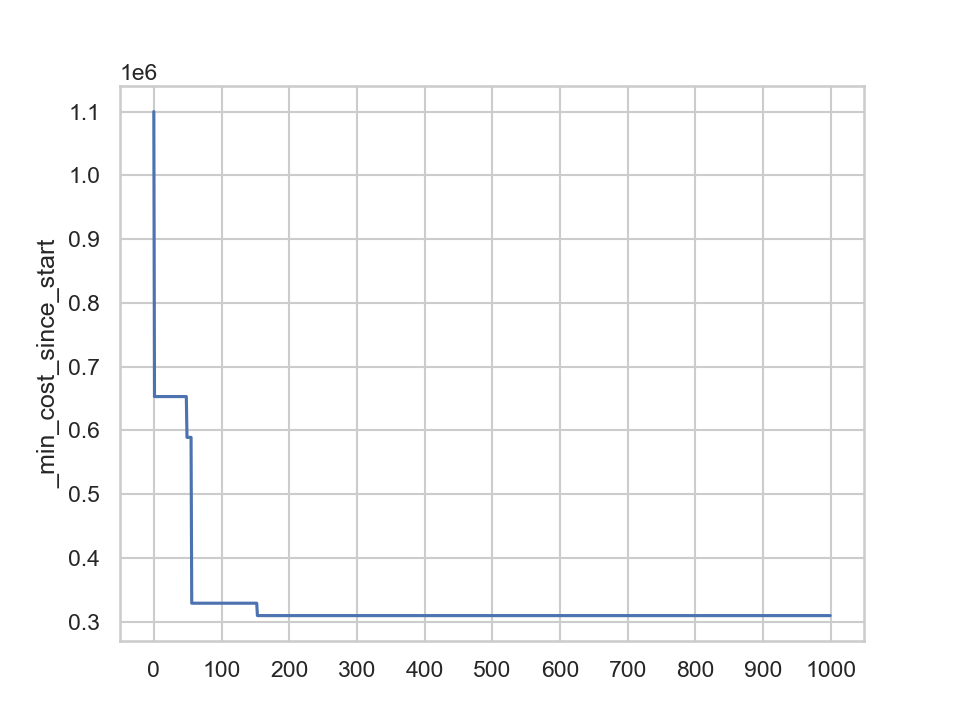
\includegraphics[scale=0.6]{figures/experiments/1000_iter/min_cost_1000.png}}
		\caption[Minimal cost]{Minimal cost found since the start.}
		\label{fig:min_cost_1000}
	\end{centering}
\end{figure}


The associated costs are depicted in Figure \ref{fig:min_cost_1000}. The minimal cost found by the algorithm declines rapidly in the first iterations and then plateaus out after a small drop at around iteration 150. This last decrease in cost was not captured by other runs, since they were capped at 100 iterations. The step-wise decrease in cost is due to a new and cheaper routing being found (drop) after which the algorithm produces only equal or worse solutions (plateau). Important to notice, is that the minimal found cost of ca. 309.000 Euro does not reflect the total cost of the network, but only the lines additionally built by the algorithm. Already existing lines do not appear in the cost function since their cost is zero. To calculate the total cost of the solution including the existing lines, all lines were considered to be newly built by the algorithm in a post processing step. This lead to a cost of 1.95M Euro. This cost can now be compared to the same calculation done with the extracted MV grid of the input. This results in costs of 2.17M Euros. The found solution of the algorithm is therefore only 89\% of the cost of the input grid.



\begin{figure}[h]
	\begin{centering}
		{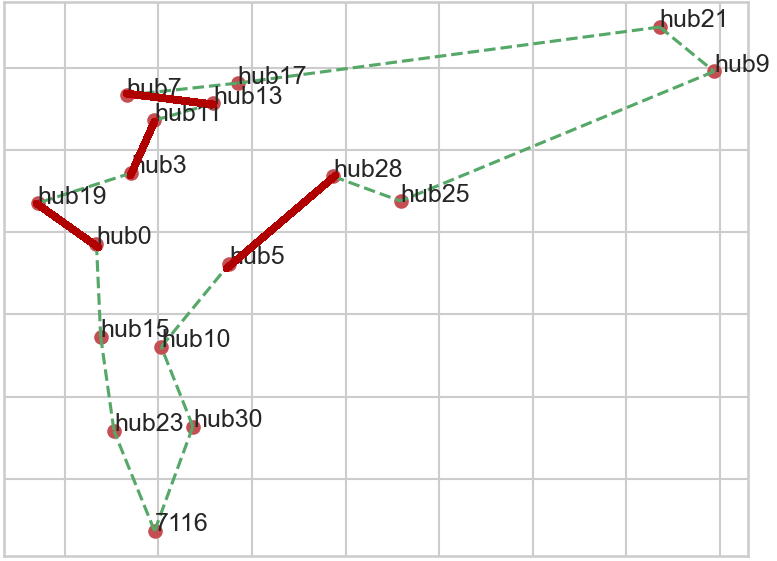
\includegraphics[scale=0.6]{figures/experiments/1000_iter/best_mv_1000.png}}
		\caption[Result grid schematic]{Schematic view of the best found MV grid. The "hubs" resemble MV/LV trafos which need to be connected to "7116" - the HV/MV trafo. Newly created lines by the algorithm are marked red.}
		\label{fig:best_mv_1000}
	\end{centering}
\end{figure}


To better see how the algorithm connects the buses a schematic view of the solution is given in Figure \ref{fig:best_mv_1000}. Here the rings structure is clearly visible. 





\subsection{Parameterstudy}
As listed in section \ref{parameters}, the algorithm has fairly many input parameters. Trying out multiple values for each parameter in all possible combinations would therefore be unfeasible. Instead, single parameters are are varied while the remaining parameters are kept at their default values. When only single parameters are varied, interactions between parameters can unfortunately not be traced anymore. \\

The parameter study is divided into four parts. First, the parameter for maximum number of stations per ring is studied (maximalRingsize). The second part investigates the parameter that changes the number of constructed solutions (antsPerColony, iterations). The third part examines the parameter controlling the expansion rule ($q0$, $\alpha$, $\beta$) and the last part studies the parameter controlling the pheromone update ($\rho$, $\xi$).

\subsubsection{Control Maximum Number of Stations per Ring}\label{stations_per_ring}
In the first part the maximal number of buses per ring are limited to a fixed value. Limiting the number of stations per ring can be useful to reduce the loading of the lines due to a smaller number of connected loads. Additionally, it decrease the number of stations being cut off electricity in case of a failure. Limiting the number of stations can be done easily during the expansion process of the ant. When an ant expands a new triangle during the solution building process, the number of stations of the ring also increases by one (neighboring triangles already share two corners). This applies to all triangles except the very first one expanded from the HV/MV transformer, where two stations are added. The number of stations per ring is therefore the number of expanded triangles incremented by one. When the ant reaches the maximum number of triangles it is allowed to expand, it stops with the expansion and starts constructing a new ring starting from the HV/MV trafo. Downwards, the maximal number of stations per ring is limited depending on the structure of the grid. The smallest number of stations per ring for which the algorithm was able to find a solution is eight. For less then eight stations per ring it is impossible to build a solution, due to the problem formulated in section \ref{sec:tri_problem}. There exist only three neighboring triangles to the start transformer and each ring occupies at least one of them. If all neighbors of the start transformer are blocked but some stations are still not connected, the ant must perform a restart. In case of maximal seven stations per ring, the ant restarted every solution building attempt out of 1500. A Manual check confirmed that it is indeed impossible for the algorithm ti find a solution.


\begin{figure}
	\centering
	\begin{minipage}{.5\textwidth}
		\centering
		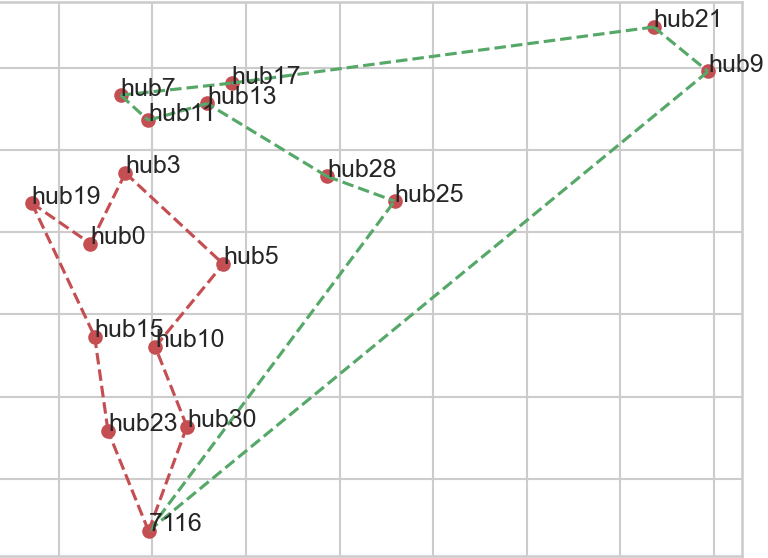
\includegraphics[width=1\linewidth]{figures/experiments/ringsize/size_8_9.png}
		\captionof{figure}[Max. 8/9 buses per ring schematic]{Max. 8/9 buses per ring.}
		\label{fig:ringsize_89}
	\end{minipage}%
	\begin{minipage}{.5\textwidth}
		\centering
		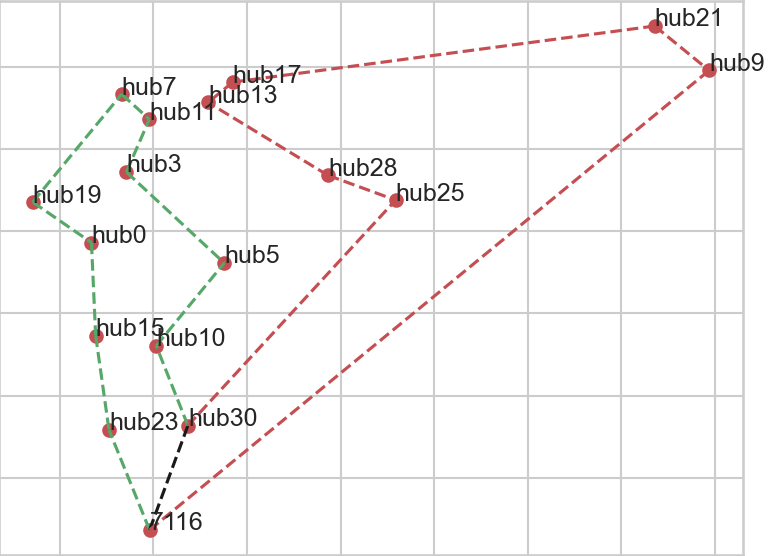
\includegraphics[width=1\linewidth]{figures/experiments/ringsize/size_10.png}
		\captionof{figure}[Max. 10 buses per ring schematic]{Max. 10 buses per ring.}
		\label{fig:ringsize_10}
	\end{minipage}
\end{figure}
Figure \ref{fig:ringsize_89} and \ref{fig:ringsize_10} show the rings being build when limiting the maximum number of stations to 8,9 and 10 in the schematic view of the map (they both can be seen in the appendix with the actual course of lines). The predicted cost of building the network as suggested in Figure \ref{fig:ringsize_89} would amount to 2.53M Euro (117 \% when compared to te original network) and 2.52M Euro (116 \%) for the network suggested in Figure \ref{fig:ringsize_10}. In general it makes sense, that increasing the number of rings also increase the cost, since additional cables are required to return to the HV/MV transformer. For more than 10 but less than 16 stations the algorithm found the same solution as shown in Figure \ref{fig:ringsize_10} and for 16 or more stations the algorithm suggested building a single ring, which is the cheapest option for this grid.

%\begin{figure}[h]
	\begin{centering}
		{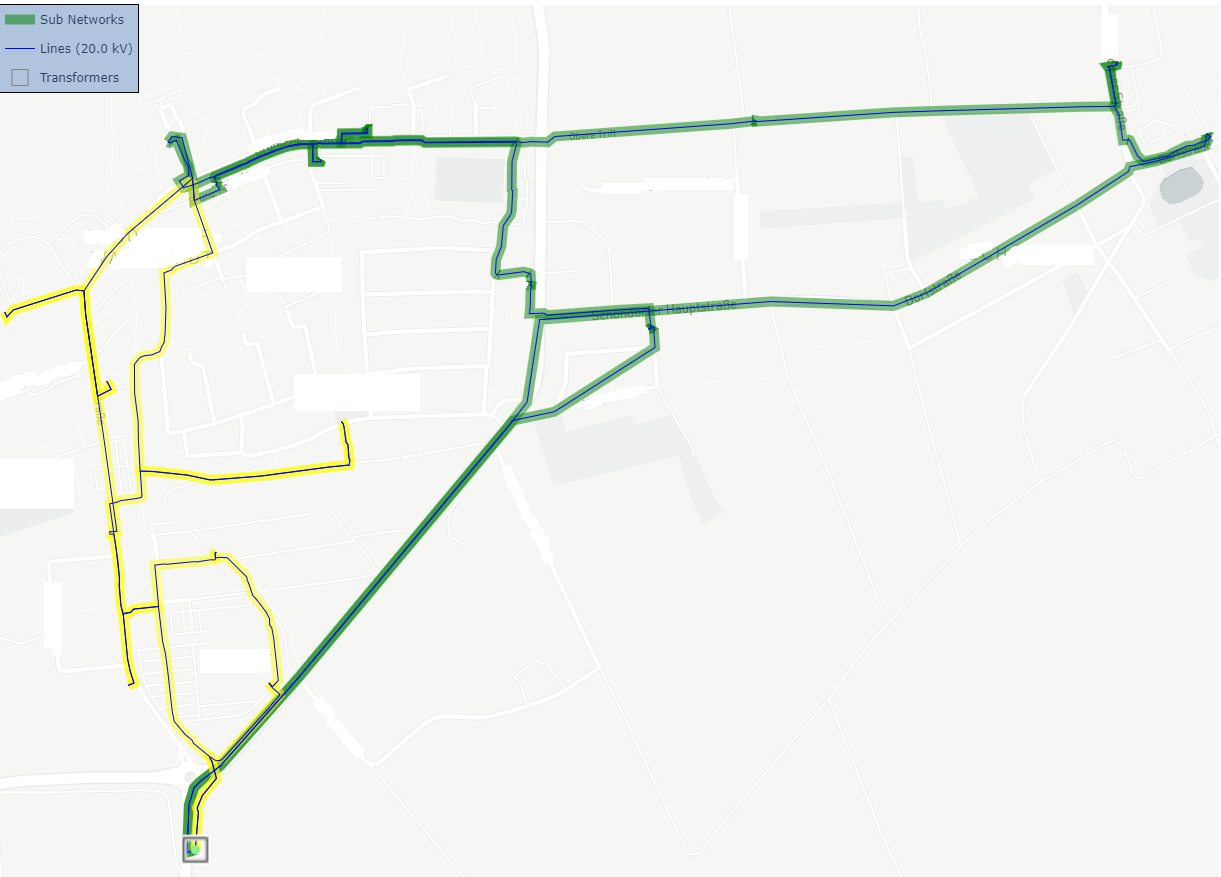
\includegraphics[scale=0.4]{figures/experiments/ringsize/ringsize89_2.png}}
		\caption{Max. 8/9 buses per ring (MV)}
		\label{fig:ringsize89_2}
	\end{centering}
\end{figure}

%\begin{figure}[h]
	\begin{centering}
		{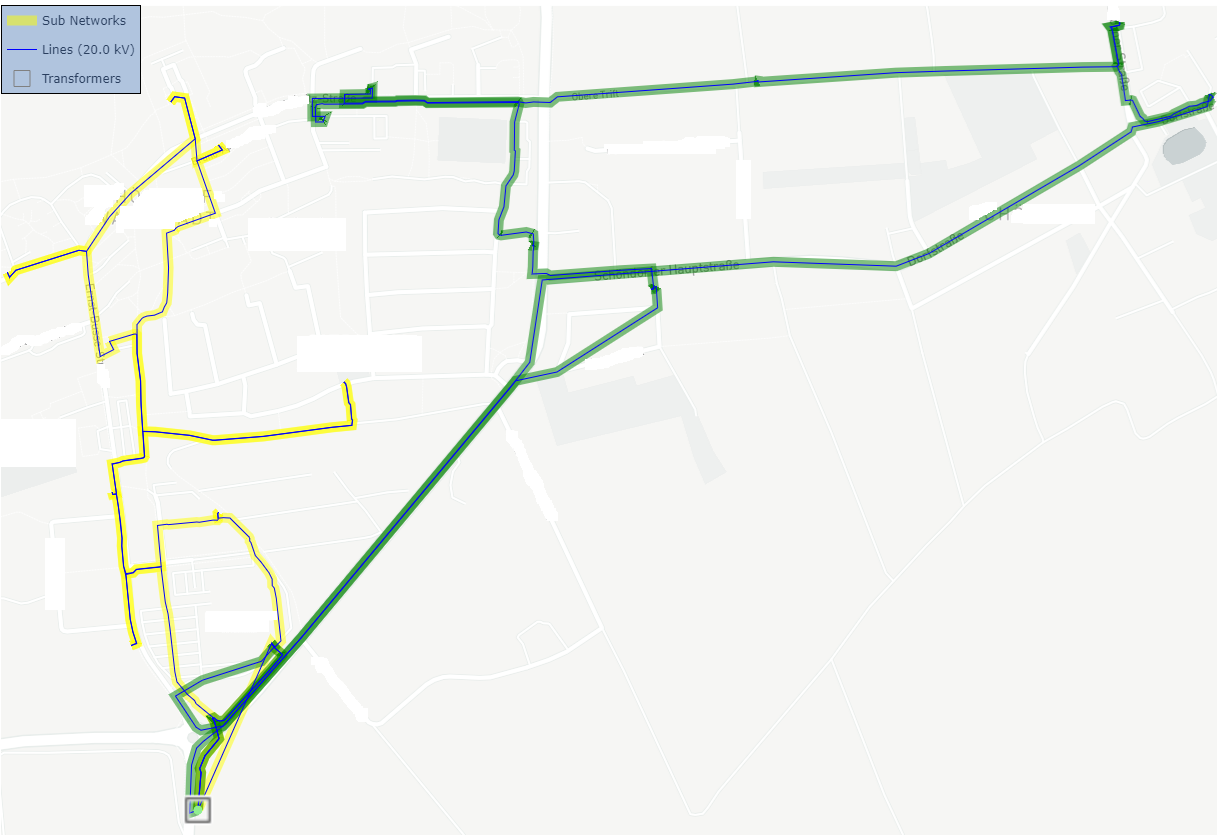
\includegraphics[scale=0.4]{figures/experiments/ringsize/ringsize10_2.png}}
		\caption{Max. ten buses per ring (MV)}
		\label{fig:ringsize10_2}
	\end{centering}
\end{figure}

%\begin{figure}[h]
	\begin{centering}
		{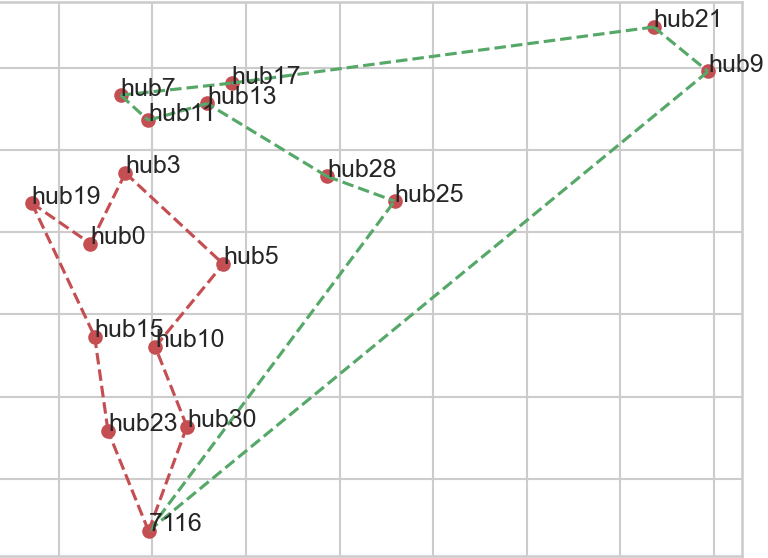
\includegraphics[scale=0.7]{figures/experiments/ringsize/size_8_9.png}}
		\caption{Schematic view of the best found MV grid with a maximum of eight or nine stations per ring.}
		\label{fig:ringsize_8_9}
	\end{centering}
\end{figure}

%\begin{figure}[h]
	\begin{centering}
		{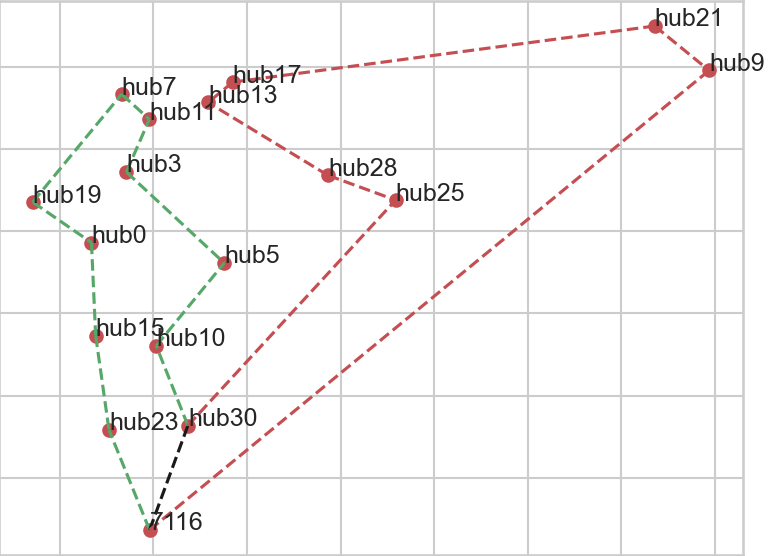
\includegraphics[scale=0.7]{figures/experiments/ringsize/size_10.png}}
		\caption{Schematic view of the best found MV grid with a maximum of ten stations per ring.}
		\label{fig:ringsize_10}
	\end{centering}
\end{figure}


\subsubsection{Control Number of Constructed Solutions}\label{constructed_solutions}

To perform well, ACO algorithms need to learn from previous iterations and explore a sufficient area of the search space. Even though the heuristic function can lead ants quickly towards reasonable results the number of constructed solutions plays a major role. \textit{Ant-Colony-System} \cite{ant_coloy_system} by Dorigo et. al. presents three parameters to control the number of constructed solutions. The number of iterations, the number of colonies and the number of ants per colony. The ants solution building process is only dependent on the best solution of the previous iteration and not on the solutions built by other ants in the same iteration. Therefore, a second independent colony of ants could create a solution in parallel. \textit{APMV} is a sequential algorithm therefore the number of colonies is always set to one. In future work the feature of multiple colonies per iteration could be added to reduce runtime. \\
How the minimal found cost change with respect to the number of iterations can already be seen in Figure \ref{fig:min_cost_1000}. On this test grid the greatest reduction in cost is already achieved after ca. 50 iterations. Around iteration 150 another small decrease in cost can be observed. Due to limited computational resources though, the default number of iterations is set to 100. An automated stop of searching for a further decrease in cost after a certain amount of iterations could be implemented.
\begin{figure}[h]
	\begin{centering}
		{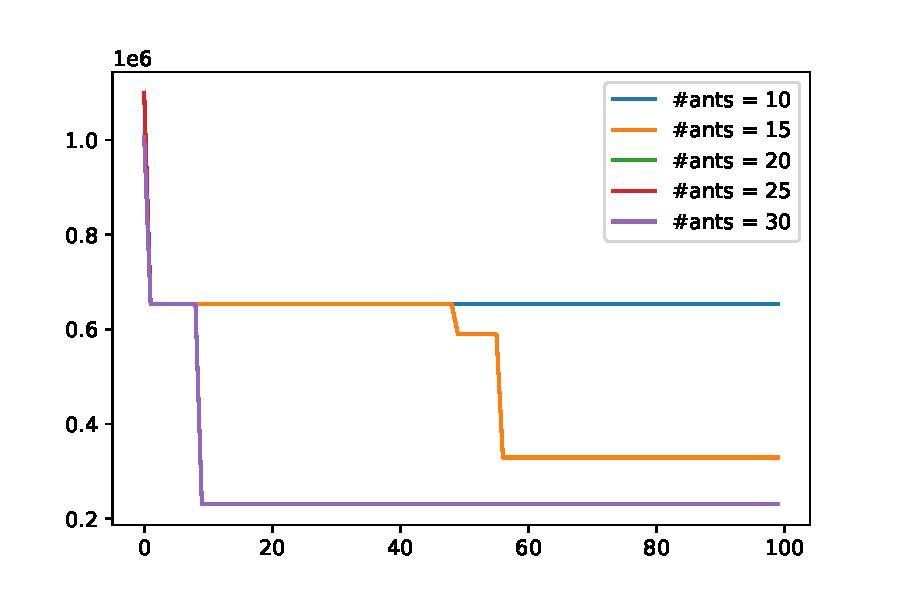
\includegraphics[scale=0.7]{figures/experiments/plt_ant.pdf}}
		\caption[Parameter study: number of ants]{Minimal cost found since the start for different number of ants per iteration.}
		\label{fig:plt_ant}
	\end{centering}
\end{figure}

The number of ants per iteration is the third parameter to control the number of constructed solutions. Its effect is shown in Figure \ref{fig:plt_ant}, which depicts the minimum cost found for different number of ants per iteration. The cost for 20 and 25 ants per iteration is congruent with the cost for 30 ants per iteration (this might be caused by the usage of the same seed in the algorithms random functions). For 20,25 and 30 ants the algorithm yields the best results. Using less ants per iteration might lead to less exploration and therefore a convergence towards a local minimum. In the future it would be interesting to increase the number of ants even further until the performance would decline again.

\subsubsection{Control Expansion Rule}\label{expansion_rule}
The parameters which control the expansion rule are $q0$, $\alpha$ and $\beta$. They guide the ant in its decision which node to expand next. The parameter $q0$ determines to which extend the ant is influenced by knowledge of the best solution of previous iterations. It modulates the trade-off between exploitation and exploration. Figure \ref{fig:q_0} shows the minimal cost found at a certain iteration with respect to different values of $q0$. For $q0 = 1$ the ant builds a solution and is forced afterwards to always expand the exact same components since no exploration is allowed. That is why the ant can never explore a better solution and therefore the costs can never decrease. The best solution is found for $q0 = 0.75$, since it enables the ant to explore more of the search space. Similar to the number of ants in the previous subsection it would interesting to investigate even lower values for $q0$ in the future until the performance of the algorithm would decline again. \\
\begin{figure}[h]
	\begin{centering}
		{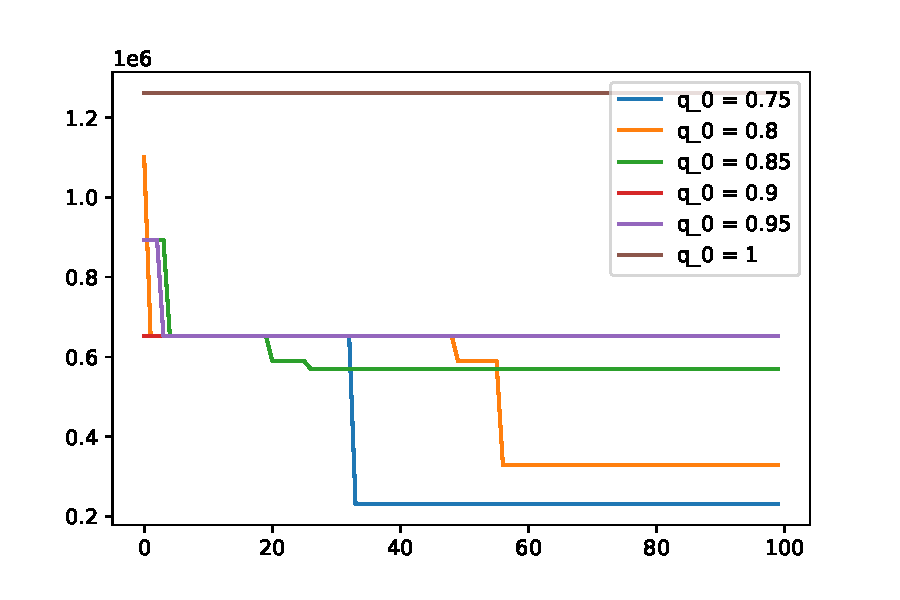
\includegraphics[scale=0.8]{figures/experiments/q_0.pdf}}
		\caption[Parameter study: $\protect q0$]{Minimal cost found since the start for different $\protect q0$.}
		\label{fig:q_0}
	\end{centering}
\end{figure}

The parameters $\alpha$ and $\beta$ describe how much the ants decision process of expanding new nodes should be guided by pheromones or heuristics.

\begin{figure}[h]
	\begin{centering}
		{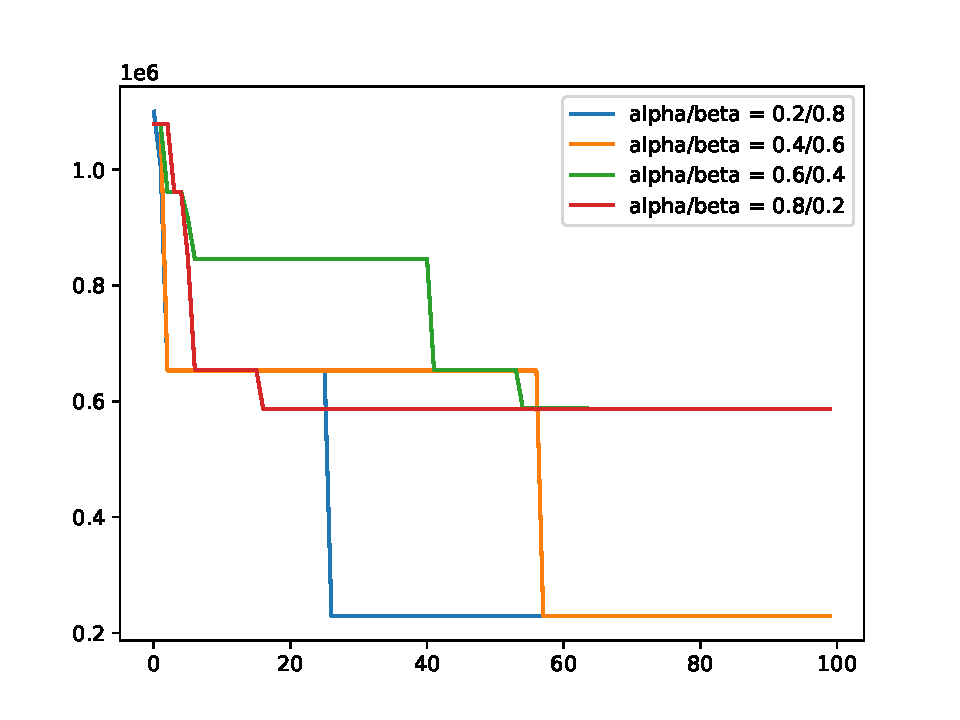
\includegraphics[scale=0.8]{figures/experiments/alpha_beta.pdf}}
		\caption{Minimal cost found since the start for different configurations of $\protect\alpha$ and $\protect\beta$.}
		\label{fig:alpha_beta}
	\end{centering}
\end{figure}

\subsubsection{Control Pheromone Update}\label{pheromone_update}

Results of different estimated min cost:
	- looks like as long as emec cost is lower than real cost the convergence is good!

\subsection{Runtime}
\subsection{Discussion}\label{sec:discussion}
\subsubsection{Triangulation and Parallel Lines}
	- kann eigentlich keine parallelen ringe. (diese sind aber anscheinend in Nutzung)
	- bessere Sicherheit ohne parallele lines?
    \chapter{Conclusion}\label{chap:conclusion}
This work gave an introduction to ant colony optimization and how it can be used in the context of medium voltage grids. The presented algorithm was tested and evaluated on a real world cross voltage example and showed good results. It found a solution, which only cost 89\% when compared to the cost of the example grid. Furthermore, the crucial triangulation step of the algorithm was examined. The benefits are a reduction of the search space which comes at the cost of not finding valid solutions in certain cases. Finally, a parameter study was conducted to understand more about the influence of certain parameters on the final result and its findings can be used to further improve the performance of the algorithm. \\

Additional improvements to the algorithm would be to develop a method to fix problematic solutions in a postprocessing step to avoid restarts and therefore speed up the algorithm. Also, the functionality of explicitly allowing or preventing the algorithm from building parallel lines could be implemented. Another way of improving the runtime would be to parallelize the algorithm via the usage of multiple independent colonies. More research is also required in comparing the performance of APMV with other grid planning algorithms. This should be done on multiple other real world examples including grids with larger size. \\

Finally, ACO seems to be a promising tool for more automated planning of electric grids in the future. 


\chapter*{Acknowledgements}
\thispagestyle{empty}

I would like to thank Janis Kähler and 

\clearpage



\appendix
\chapter{Appendix}

\begin{figure}[h]
	\begin{centering}
		{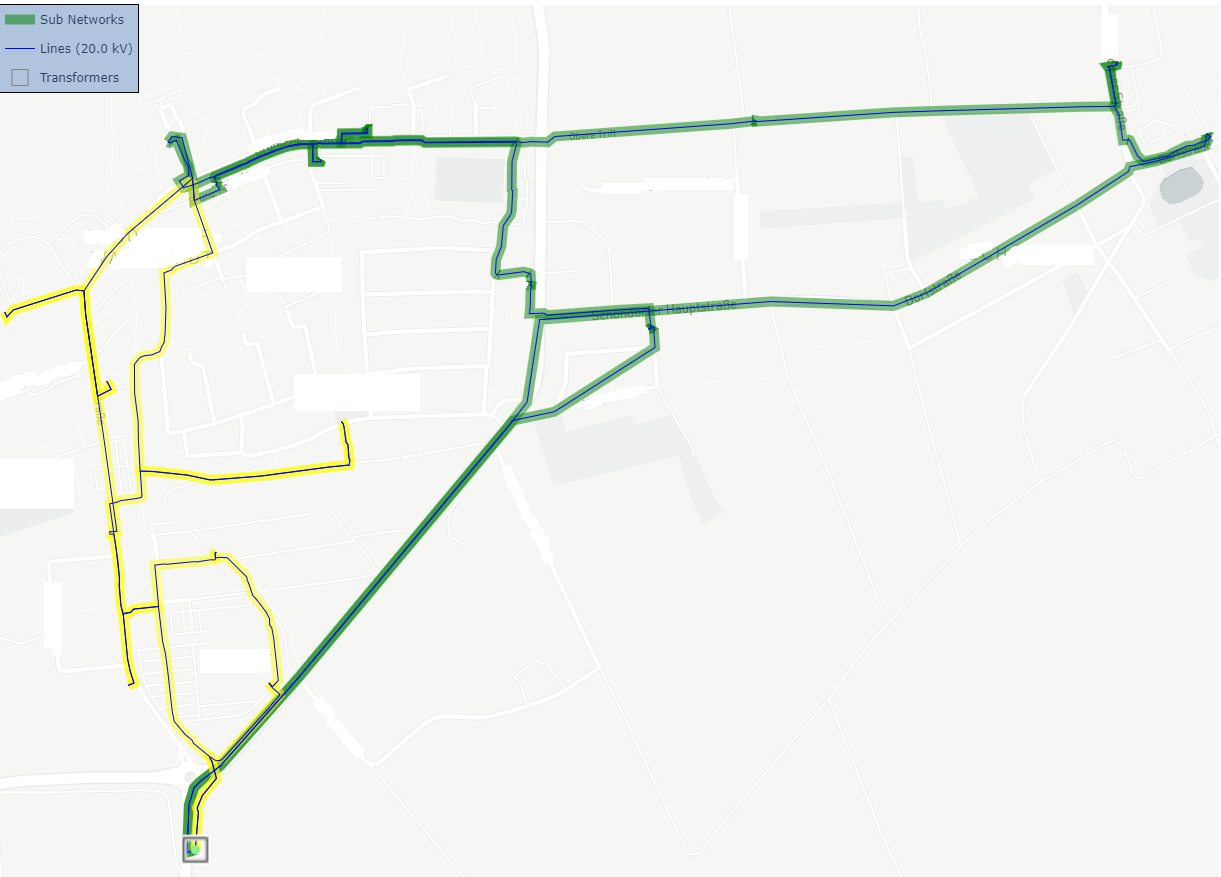
\includegraphics[scale=0.4]{figures/experiments/ringsize/ringsize89_2.png}}
		\caption{Max. 8/9 buses per ring (MV)}
		\label{fig:ringsize89_2}
	\end{centering}
\end{figure}

\begin{figure}[h]
	\begin{centering}
		{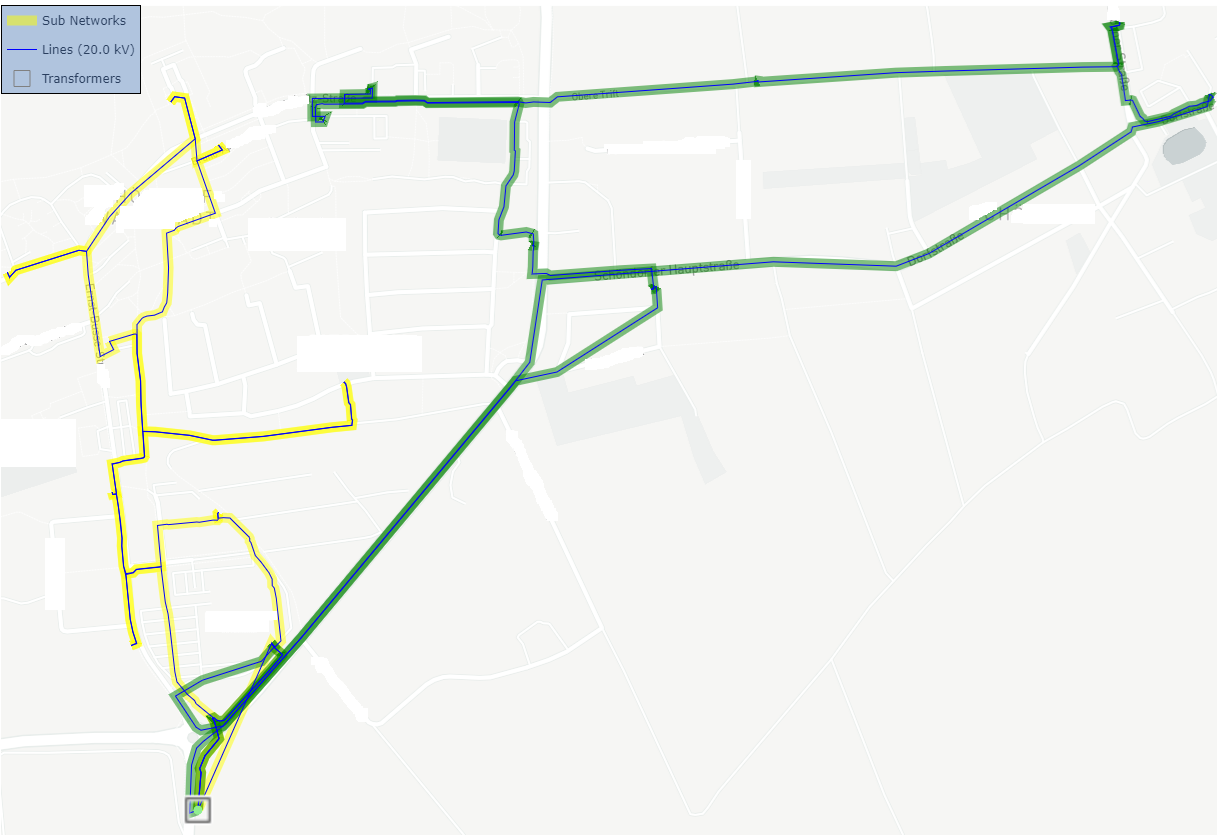
\includegraphics[scale=0.4]{figures/experiments/ringsize/ringsize10_2.png}}
		\caption{Max. ten buses per ring (MV)}
		\label{fig:ringsize10_2}
	\end{centering}
\end{figure}

    
    % If you want a list of your ToDos at the end of the document
    % don't forget to remove before submission!
    %% place it somewhere in the document
\chapter*{ToDo Counters}
\newcounter{ct}%
To Dos: \arabic{todos}; \hspace{1em}%
\setcounter{ct}{0}%
\whiledo {\value{ct} < \value{todos}}%
{%
	\stepcounter {ct}%
    \ref{todo \thect}%
	\ifnum\value{ct} = \value{todos}{}\else{, }\fi
}

Parts to extend: \arabic{extends}; \hspace{1em}%
\setcounter{ct}{0}%
\whiledo {\value{ct} < \value{extends}}%
{%
	\stepcounter {ct}%
	\ref{extend \thect}%
	\ifnum\value{ct} = \value{extends}{}\else{, }\fi
}

Draft parts: \arabic{drafts}; \hspace{1em}%
\setcounter{ct}{0}%
\whiledo {\value{ct} < \value{drafts}}%
{%
	\stepcounter {ct}%
	\ref{draft \thect}%
	\ifnum\value{ct} = \value{drafts}{}\else{, }\fi
}


    \bibliographystyle{ieeetr}
    \bibliography{bib/topic1,bib/topic2}
    % bibliography is not in the table of contents per default, add it manually
    % enable the \renewcommand for german header
    % \renewcommand{\bibname}{Literaturverzeichnis}
    \addcontentsline{toc}{chapter}{Bibliography}
    \newpage
    \thispagestyle{empty}
    \mbox{}


\end{document}
